% Options for packages loaded elsewhere
\PassOptionsToPackage{unicode}{hyperref}
\PassOptionsToPackage{hyphens}{url}
%
\documentclass[
]{article}
\usepackage{amsmath,amssymb}
\usepackage{iftex}
\ifPDFTeX
  \usepackage[T1]{fontenc}
  \usepackage[utf8]{inputenc}
  \usepackage{textcomp} % provide euro and other symbols
\else % if luatex or xetex
  \usepackage{unicode-math} % this also loads fontspec
  \defaultfontfeatures{Scale=MatchLowercase}
  \defaultfontfeatures[\rmfamily]{Ligatures=TeX,Scale=1}
\fi
\usepackage{lmodern}
\ifPDFTeX\else
  % xetex/luatex font selection
\fi
% Use upquote if available, for straight quotes in verbatim environments
\IfFileExists{upquote.sty}{\usepackage{upquote}}{}
\IfFileExists{microtype.sty}{% use microtype if available
  \usepackage[]{microtype}
  \UseMicrotypeSet[protrusion]{basicmath} % disable protrusion for tt fonts
}{}
\makeatletter
\@ifundefined{KOMAClassName}{% if non-KOMA class
  \IfFileExists{parskip.sty}{%
    \usepackage{parskip}
  }{% else
    \setlength{\parindent}{0pt}
    \setlength{\parskip}{6pt plus 2pt minus 1pt}}
}{% if KOMA class
  \KOMAoptions{parskip=half}}
\makeatother
\usepackage{xcolor}
\usepackage[margin=1in]{geometry}
\usepackage{color}
\usepackage{fancyvrb}
\newcommand{\VerbBar}{|}
\newcommand{\VERB}{\Verb[commandchars=\\\{\}]}
\DefineVerbatimEnvironment{Highlighting}{Verbatim}{commandchars=\\\{\}}
% Add ',fontsize=\small' for more characters per line
\usepackage{framed}
\definecolor{shadecolor}{RGB}{248,248,248}
\newenvironment{Shaded}{\begin{snugshade}}{\end{snugshade}}
\newcommand{\AlertTok}[1]{\textcolor[rgb]{0.94,0.16,0.16}{#1}}
\newcommand{\AnnotationTok}[1]{\textcolor[rgb]{0.56,0.35,0.01}{\textbf{\textit{#1}}}}
\newcommand{\AttributeTok}[1]{\textcolor[rgb]{0.13,0.29,0.53}{#1}}
\newcommand{\BaseNTok}[1]{\textcolor[rgb]{0.00,0.00,0.81}{#1}}
\newcommand{\BuiltInTok}[1]{#1}
\newcommand{\CharTok}[1]{\textcolor[rgb]{0.31,0.60,0.02}{#1}}
\newcommand{\CommentTok}[1]{\textcolor[rgb]{0.56,0.35,0.01}{\textit{#1}}}
\newcommand{\CommentVarTok}[1]{\textcolor[rgb]{0.56,0.35,0.01}{\textbf{\textit{#1}}}}
\newcommand{\ConstantTok}[1]{\textcolor[rgb]{0.56,0.35,0.01}{#1}}
\newcommand{\ControlFlowTok}[1]{\textcolor[rgb]{0.13,0.29,0.53}{\textbf{#1}}}
\newcommand{\DataTypeTok}[1]{\textcolor[rgb]{0.13,0.29,0.53}{#1}}
\newcommand{\DecValTok}[1]{\textcolor[rgb]{0.00,0.00,0.81}{#1}}
\newcommand{\DocumentationTok}[1]{\textcolor[rgb]{0.56,0.35,0.01}{\textbf{\textit{#1}}}}
\newcommand{\ErrorTok}[1]{\textcolor[rgb]{0.64,0.00,0.00}{\textbf{#1}}}
\newcommand{\ExtensionTok}[1]{#1}
\newcommand{\FloatTok}[1]{\textcolor[rgb]{0.00,0.00,0.81}{#1}}
\newcommand{\FunctionTok}[1]{\textcolor[rgb]{0.13,0.29,0.53}{\textbf{#1}}}
\newcommand{\ImportTok}[1]{#1}
\newcommand{\InformationTok}[1]{\textcolor[rgb]{0.56,0.35,0.01}{\textbf{\textit{#1}}}}
\newcommand{\KeywordTok}[1]{\textcolor[rgb]{0.13,0.29,0.53}{\textbf{#1}}}
\newcommand{\NormalTok}[1]{#1}
\newcommand{\OperatorTok}[1]{\textcolor[rgb]{0.81,0.36,0.00}{\textbf{#1}}}
\newcommand{\OtherTok}[1]{\textcolor[rgb]{0.56,0.35,0.01}{#1}}
\newcommand{\PreprocessorTok}[1]{\textcolor[rgb]{0.56,0.35,0.01}{\textit{#1}}}
\newcommand{\RegionMarkerTok}[1]{#1}
\newcommand{\SpecialCharTok}[1]{\textcolor[rgb]{0.81,0.36,0.00}{\textbf{#1}}}
\newcommand{\SpecialStringTok}[1]{\textcolor[rgb]{0.31,0.60,0.02}{#1}}
\newcommand{\StringTok}[1]{\textcolor[rgb]{0.31,0.60,0.02}{#1}}
\newcommand{\VariableTok}[1]{\textcolor[rgb]{0.00,0.00,0.00}{#1}}
\newcommand{\VerbatimStringTok}[1]{\textcolor[rgb]{0.31,0.60,0.02}{#1}}
\newcommand{\WarningTok}[1]{\textcolor[rgb]{0.56,0.35,0.01}{\textbf{\textit{#1}}}}
\usepackage{graphicx}
\makeatletter
\def\maxwidth{\ifdim\Gin@nat@width>\linewidth\linewidth\else\Gin@nat@width\fi}
\def\maxheight{\ifdim\Gin@nat@height>\textheight\textheight\else\Gin@nat@height\fi}
\makeatother
% Scale images if necessary, so that they will not overflow the page
% margins by default, and it is still possible to overwrite the defaults
% using explicit options in \includegraphics[width, height, ...]{}
\setkeys{Gin}{width=\maxwidth,height=\maxheight,keepaspectratio}
% Set default figure placement to htbp
\makeatletter
\def\fps@figure{htbp}
\makeatother
\setlength{\emergencystretch}{3em} % prevent overfull lines
\providecommand{\tightlist}{%
  \setlength{\itemsep}{0pt}\setlength{\parskip}{0pt}}
\setcounter{secnumdepth}{-\maxdimen} % remove section numbering
\ifLuaTeX
  \usepackage{selnolig}  % disable illegal ligatures
\fi
\IfFileExists{bookmark.sty}{\usepackage{bookmark}}{\usepackage{hyperref}}
\IfFileExists{xurl.sty}{\usepackage{xurl}}{} % add URL line breaks if available
\urlstyle{same}
\hypersetup{
  pdftitle={Reads and plots data from the Manuscript Marreiros et al.~2024},
  pdfauthor={Mae Goder-Goldberger, Joao Marreiros, Eduardo Paixao, Erella Hovers},
  hidelinks,
  pdfcreator={LaTeX via pandoc}}

\title{Reads and plots data from the Manuscript Marreiros et al.~2024}
\author{Mae Goder-Goldberger, Joao Marreiros, Eduardo Paixao, Erella
Hovers}
\date{2024-06-06 21:17:00.692528}

\begin{document}
\maketitle

\textbf{Brief description of the script}

\hypertarget{content}{%
\section{Content}\label{content}}

This script reads and plots the data from the 3D and 2D morphometric
analysis of the artefacts' engraved incisions. For details on the
methods and data acquisition, please visit the Materials and Methods
section of the paper.

The knit directory for this script is the project directory.This R
project and respective scripts follow the procedures described by
Marwick et al.~2017.

For any questions, comments and inputs, please contact:

João Marreiros,
\href{mailto:joao.marreiros@leiza.de}{\nolinkurl{joao.marreiros@leiza.de}}

\hypertarget{load-packages}{%
\section{Load packages}\label{load-packages}}

\begin{Shaded}
\begin{Highlighting}[]
\FunctionTok{library}\NormalTok{(R.utils)}
\end{Highlighting}
\end{Shaded}

\begin{verbatim}
## Warning: package 'R.utils' was built under R version 4.3.1
\end{verbatim}

\begin{verbatim}
## Loading required package: R.oo
\end{verbatim}

\begin{verbatim}
## Loading required package: R.methodsS3
\end{verbatim}

\begin{verbatim}
## R.methodsS3 v1.8.2 (2022-06-13 22:00:14 UTC) successfully loaded. See ?R.methodsS3 for help.
\end{verbatim}

\begin{verbatim}
## R.oo v1.25.0 (2022-06-12 02:20:02 UTC) successfully loaded. See ?R.oo for help.
\end{verbatim}

\begin{verbatim}
## 
## Attaching package: 'R.oo'
\end{verbatim}

\begin{verbatim}
## The following object is masked from 'package:R.methodsS3':
## 
##     throw
\end{verbatim}

\begin{verbatim}
## The following objects are masked from 'package:methods':
## 
##     getClasses, getMethods
\end{verbatim}

\begin{verbatim}
## The following objects are masked from 'package:base':
## 
##     attach, detach, load, save
\end{verbatim}

\begin{verbatim}
## R.utils v2.12.3 (2023-11-18 01:00:02 UTC) successfully loaded. See ?R.utils for help.
\end{verbatim}

\begin{verbatim}
## 
## Attaching package: 'R.utils'
\end{verbatim}

\begin{verbatim}
## The following object is masked from 'package:utils':
## 
##     timestamp
\end{verbatim}

\begin{verbatim}
## The following objects are masked from 'package:base':
## 
##     cat, commandArgs, getOption, isOpen, nullfile, parse, warnings
\end{verbatim}

\begin{Shaded}
\begin{Highlighting}[]
\FunctionTok{library}\NormalTok{(ggplot2)}
\end{Highlighting}
\end{Shaded}

\begin{verbatim}
## Warning: package 'ggplot2' was built under R version 4.3.1
\end{verbatim}

\begin{Shaded}
\begin{Highlighting}[]
\FunctionTok{library}\NormalTok{(tools)}
\FunctionTok{library}\NormalTok{(tidyverse)}
\end{Highlighting}
\end{Shaded}

\begin{verbatim}
## Warning: package 'readr' was built under R version 4.3.1
\end{verbatim}

\begin{verbatim}
## Warning: package 'dplyr' was built under R version 4.3.1
\end{verbatim}

\begin{verbatim}
## Warning: package 'stringr' was built under R version 4.3.1
\end{verbatim}

\begin{verbatim}
## Warning: package 'lubridate' was built under R version 4.3.1
\end{verbatim}

\begin{verbatim}
## -- Attaching core tidyverse packages ------------------------ tidyverse 2.0.0 --
## v dplyr     1.1.4     v readr     2.1.5
## v forcats   1.0.0     v stringr   1.5.1
## v lubridate 1.9.3     v tibble    3.2.1
## v purrr     1.0.2     v tidyr     1.3.0
\end{verbatim}

\begin{verbatim}
## -- Conflicts ------------------------------------------ tidyverse_conflicts() --
## x tidyr::extract() masks R.utils::extract()
## x dplyr::filter()  masks stats::filter()
## x dplyr::lag()     masks stats::lag()
## i Use the conflicted package (<http://conflicted.r-lib.org/>) to force all conflicts to become errors
\end{verbatim}

\begin{Shaded}
\begin{Highlighting}[]
\FunctionTok{library}\NormalTok{(doBy)}
\end{Highlighting}
\end{Shaded}

\begin{verbatim}
## Warning: package 'doBy' was built under R version 4.3.1
\end{verbatim}

\begin{verbatim}
## 
## Attaching package: 'doBy'
## 
## The following object is masked from 'package:dplyr':
## 
##     order_by
\end{verbatim}

\begin{Shaded}
\begin{Highlighting}[]
\FunctionTok{library}\NormalTok{(ggrepel)}
\end{Highlighting}
\end{Shaded}

\begin{verbatim}
## Warning: package 'ggrepel' was built under R version 4.3.1
\end{verbatim}

\begin{Shaded}
\begin{Highlighting}[]
\FunctionTok{library}\NormalTok{(flextable)}
\end{Highlighting}
\end{Shaded}

\begin{verbatim}
## Warning: package 'flextable' was built under R version 4.3.1
\end{verbatim}

\begin{verbatim}
## 
## Attaching package: 'flextable'
## 
## The following object is masked from 'package:purrr':
## 
##     compose
\end{verbatim}

\begin{Shaded}
\begin{Highlighting}[]
\FunctionTok{library}\NormalTok{(readr)}
\FunctionTok{library}\NormalTok{(ggpubr)}
\end{Highlighting}
\end{Shaded}

\begin{verbatim}
## 
## Attaching package: 'ggpubr'
## 
## The following objects are masked from 'package:flextable':
## 
##     border, font, rotate
\end{verbatim}

\begin{Shaded}
\begin{Highlighting}[]
\FunctionTok{library}\NormalTok{(crosstable)}
\end{Highlighting}
\end{Shaded}

\begin{verbatim}
## Warning: package 'crosstable' was built under R version 4.3.1
\end{verbatim}

\begin{verbatim}
## 
## Attaching package: 'crosstable'
## 
## The following object is masked from 'package:purrr':
## 
##     compact
\end{verbatim}

\begin{Shaded}
\begin{Highlighting}[]
\FunctionTok{library}\NormalTok{(car)}
\end{Highlighting}
\end{Shaded}

\begin{verbatim}
## Loading required package: carData
## 
## Attaching package: 'car'
## 
## The following object is masked from 'package:dplyr':
## 
##     recode
## 
## The following object is masked from 'package:purrr':
## 
##     some
\end{verbatim}

\hypertarget{import-and-preview-data}{%
\section{Import and preview data}\label{import-and-preview-data}}

\begin{Shaded}
\begin{Highlighting}[]
\NormalTok{db }\OtherTok{\textless{}{-}} \FunctionTok{read.csv}\NormalTok{(}\StringTok{"../raw\_data/data.csv"}\NormalTok{, }\AttributeTok{stringsAsFactors=}\ConstantTok{FALSE}\NormalTok{, }\AttributeTok{sep=}\StringTok{";"}\NormalTok{, }\AttributeTok{dec=}\StringTok{"."}\NormalTok{)}

\FunctionTok{str}\NormalTok{(db)}
\end{Highlighting}
\end{Shaded}

\begin{verbatim}
## 'data.frame':    324 obs. of  8 variables:
##  $ site              : chr  "Amud1" "Qafzeh" "Amud1" "Amud1" ...
##  $ aoi               : int  1 2 1 2 1 1 1 2 1 2 ...
##  $ incision          : int  11 3 20 8 11 4 20 10 8 9 ...
##  $ profile           : int  2 2 1 1 1 3 3 2 3 3 ...
##  $ horizontaldistance: num  253 973 300 293 261 ...
##  $ maximumdepth      : num  10.62 9.05 11.61 12.49 14.43 ...
##  $ holearea          : int  1366 1378 1710 1718 1877 2043 2048 2110 2124 2237 ...
##  $ angle             : num  163 148 167 162 162 ...
\end{verbatim}

\begin{Shaded}
\begin{Highlighting}[]
\FunctionTok{head}\NormalTok{(db)}
\end{Highlighting}
\end{Shaded}

\begin{verbatim}
##     site aoi incision profile horizontaldistance maximumdepth holearea angle
## 1  Amud1   1       11       2              253.2        10.62     1366 163.1
## 2 Qafzeh   2        3       2              973.1         9.05     1378 148.2
## 3  Amud1   1       20       1              300.3        11.61     1710 167.1
## 4  Amud1   2        8       1              293.2        12.49     1718 161.8
## 5  Amud1   1       11       1              261.4        14.43     1877 162.5
## 6  Amud1   1        4       3              277.0        16.01     2043 158.3
\end{verbatim}

\hypertarget{import-and-summarize-data}{%
\section{Import and summarize data}\label{import-and-summarize-data}}

\begin{Shaded}
\begin{Highlighting}[]
\CommentTok{\# summarise data frome ach artefact, organised by AOI}

\CommentTok{\# sample data per artefact}

\NormalTok{manotdb }\OtherTok{\textless{}{-}} \FunctionTok{filter}\NormalTok{(db, site }\SpecialCharTok{==} \StringTok{"Manot"}\NormalTok{)}
\NormalTok{amud1db }\OtherTok{\textless{}{-}} \FunctionTok{filter}\NormalTok{(db, site }\SpecialCharTok{==} \StringTok{"Amud1"}\NormalTok{)}
\NormalTok{amud2db }\OtherTok{\textless{}{-}} \FunctionTok{filter}\NormalTok{(db, site }\SpecialCharTok{==} \StringTok{"Amud2"}\NormalTok{)}
\NormalTok{qzdb }\OtherTok{\textless{}{-}} \FunctionTok{filter}\NormalTok{(db, site }\SpecialCharTok{==}\StringTok{"Qafzeh"}\NormalTok{)}
\NormalTok{qnrtdb }\OtherTok{\textless{}{-}} \FunctionTok{filter}\NormalTok{(db, site }\SpecialCharTok{==}\StringTok{"Quneitra"}\NormalTok{)}

\CommentTok{\# Manot}
\CommentTok{\# Horizontal distance}
\NormalTok{manotdistance }\OtherTok{\textless{}{-}}\NormalTok{ manotdb }\SpecialCharTok{\%\textgreater{}\%} \FunctionTok{group\_by}\NormalTok{(aoi) }\SpecialCharTok{\%\textgreater{}\%}
      \FunctionTok{summarise}\NormalTok{(}
      \AttributeTok{count =} \FunctionTok{n}\NormalTok{(),}
      \AttributeTok{max =} \FunctionTok{max}\NormalTok{(horizontaldistance, }\AttributeTok{na.rm =} \ConstantTok{TRUE}\NormalTok{),}
      \AttributeTok{min =} \FunctionTok{min}\NormalTok{ (horizontaldistance, }\AttributeTok{na.rm =} \ConstantTok{TRUE}\NormalTok{),}
      \AttributeTok{mean =} \FunctionTok{mean}\NormalTok{(horizontaldistance, }\AttributeTok{na.rm =} \ConstantTok{TRUE}\NormalTok{),}
      \AttributeTok{sd =} \FunctionTok{sd}\NormalTok{(horizontaldistance, }\AttributeTok{na.rm =} \ConstantTok{TRUE}\NormalTok{),}
      \AttributeTok{median =} \FunctionTok{median}\NormalTok{(horizontaldistance, }\AttributeTok{na.rm =} \ConstantTok{TRUE}\NormalTok{),}
\NormalTok{  ) }

\CommentTok{\# Depth}
\NormalTok{manotdepth }\OtherTok{\textless{}{-}}\NormalTok{ manotdb }\SpecialCharTok{\%\textgreater{}\%} \FunctionTok{group\_by}\NormalTok{(aoi) }\SpecialCharTok{\%\textgreater{}\%}
      \FunctionTok{summarise}\NormalTok{(}
      \AttributeTok{count =} \FunctionTok{n}\NormalTok{(),}
      \AttributeTok{max =} \FunctionTok{max}\NormalTok{(maximumdepth, }\AttributeTok{na.rm =} \ConstantTok{TRUE}\NormalTok{),}
      \AttributeTok{min =} \FunctionTok{min}\NormalTok{ (maximumdepth, }\AttributeTok{na.rm =} \ConstantTok{TRUE}\NormalTok{),}
      \AttributeTok{mean =} \FunctionTok{mean}\NormalTok{(maximumdepth, }\AttributeTok{na.rm =} \ConstantTok{TRUE}\NormalTok{),}
      \AttributeTok{sd =} \FunctionTok{sd}\NormalTok{(maximumdepth, }\AttributeTok{na.rm =} \ConstantTok{TRUE}\NormalTok{),}
      \AttributeTok{median =} \FunctionTok{median}\NormalTok{(maximumdepth, }\AttributeTok{na.rm =} \ConstantTok{TRUE}\NormalTok{),}
\NormalTok{  ) }

\CommentTok{\# Area}
\NormalTok{manotarea }\OtherTok{\textless{}{-}}\NormalTok{ manotdb }\SpecialCharTok{\%\textgreater{}\%} \FunctionTok{group\_by}\NormalTok{(aoi) }\SpecialCharTok{\%\textgreater{}\%}
      \FunctionTok{summarise}\NormalTok{(}
      \AttributeTok{count =} \FunctionTok{n}\NormalTok{(),}
      \AttributeTok{max =} \FunctionTok{max}\NormalTok{(holearea, }\AttributeTok{na.rm =} \ConstantTok{TRUE}\NormalTok{),}
      \AttributeTok{min =} \FunctionTok{min}\NormalTok{ (holearea, }\AttributeTok{na.rm =} \ConstantTok{TRUE}\NormalTok{),}
      \AttributeTok{mean =} \FunctionTok{mean}\NormalTok{(holearea, }\AttributeTok{na.rm =} \ConstantTok{TRUE}\NormalTok{),}
      \AttributeTok{sd =} \FunctionTok{sd}\NormalTok{(holearea, }\AttributeTok{na.rm =} \ConstantTok{TRUE}\NormalTok{),}
      \AttributeTok{median =} \FunctionTok{median}\NormalTok{(holearea, }\AttributeTok{na.rm =} \ConstantTok{TRUE}\NormalTok{),}
\NormalTok{  ) }

\CommentTok{\# Angle}
\NormalTok{manotangle }\OtherTok{\textless{}{-}}\NormalTok{ manotdb }\SpecialCharTok{\%\textgreater{}\%} \FunctionTok{group\_by}\NormalTok{(aoi) }\SpecialCharTok{\%\textgreater{}\%}
      \FunctionTok{summarise}\NormalTok{(}
      \AttributeTok{count =} \FunctionTok{n}\NormalTok{(),}
      \AttributeTok{max =} \FunctionTok{max}\NormalTok{(angle, }\AttributeTok{na.rm =} \ConstantTok{TRUE}\NormalTok{),}
      \AttributeTok{min =} \FunctionTok{min}\NormalTok{ (angle, }\AttributeTok{na.rm =} \ConstantTok{TRUE}\NormalTok{),}
      \AttributeTok{mean =} \FunctionTok{mean}\NormalTok{(angle, }\AttributeTok{na.rm =} \ConstantTok{TRUE}\NormalTok{),}
      \AttributeTok{sd =} \FunctionTok{sd}\NormalTok{(angle, }\AttributeTok{na.rm =} \ConstantTok{TRUE}\NormalTok{),}
      \AttributeTok{median =} \FunctionTok{median}\NormalTok{(angle, }\AttributeTok{na.rm =} \ConstantTok{TRUE}\NormalTok{),}
\NormalTok{  ) }

\CommentTok{\# see data summary}
\NormalTok{manotdistance}
\end{Highlighting}
\end{Shaded}

\begin{verbatim}
## # A tibble: 3 x 7
##     aoi count   max   min  mean    sd median
##   <int> <int> <dbl> <dbl> <dbl> <dbl>  <dbl>
## 1     1     9  929.  690.  826.  82.1   814.
## 2     2    12  891.  803.  848.  33.3   848.
## 3     3    42 1163.  587.  811. 125.    816.
\end{verbatim}

\begin{Shaded}
\begin{Highlighting}[]
\NormalTok{manotdepth}
\end{Highlighting}
\end{Shaded}

\begin{verbatim}
## # A tibble: 3 x 7
##     aoi count   max   min  mean    sd median
##   <int> <int> <dbl> <dbl> <dbl> <dbl>  <dbl>
## 1     1     9  76.5  51.0  62.4  9.11   57.4
## 2     2    12  59.1  44.4  52.3  4.14   53.4
## 3     3    42 120.   25.5  64.8 21.1    61.6
\end{verbatim}

\begin{Shaded}
\begin{Highlighting}[]
\NormalTok{manotarea}
\end{Highlighting}
\end{Shaded}

\begin{verbatim}
## # A tibble: 3 x 7
##     aoi count   max   min   mean     sd median
##   <int> <int> <int> <int>  <dbl>  <dbl>  <dbl>
## 1     1     9 34240 10820 25592.  7255. 24590 
## 2     2    12 33056  9471 20100. 10597. 18449 
## 3     3    42 60785 12293 29378. 10877. 26268.
\end{verbatim}

\begin{Shaded}
\begin{Highlighting}[]
\NormalTok{manotangle}
\end{Highlighting}
\end{Shaded}

\begin{verbatim}
## # A tibble: 3 x 7
##     aoi count   max   min  mean    sd median
##   <int> <int> <dbl> <dbl> <dbl> <dbl>  <dbl>
## 1     1     9  158.  143.  150.  5.27   151.
## 2     2    12  153.  147   151.  1.65   151 
## 3     3    42  160.  136   148.  5.95   148.
\end{verbatim}

\begin{Shaded}
\begin{Highlighting}[]
\CommentTok{\# save the results }
\FunctionTok{write\_csv}\NormalTok{(manotdepth, }\StringTok{"../summary\_stats/manotdepth.csv"}\NormalTok{)}
\FunctionTok{write\_csv}\NormalTok{(manotarea, }\StringTok{"../summary\_stats/manotarea.csv"}\NormalTok{)}
\FunctionTok{write\_csv}\NormalTok{(manotangle, }\StringTok{"../summary\_stats/manotangle.csv"}\NormalTok{)}
\FunctionTok{write\_csv}\NormalTok{(manotdistance, }\StringTok{"../summary\_stats/manotdistance.csv"}\NormalTok{)}

\CommentTok{\# Amud1}
\CommentTok{\# Horizontal distance}
\NormalTok{amud1distance }\OtherTok{\textless{}{-}}\NormalTok{ amud1db }\SpecialCharTok{\%\textgreater{}\%} \FunctionTok{group\_by}\NormalTok{(aoi) }\SpecialCharTok{\%\textgreater{}\%}
      \FunctionTok{summarise}\NormalTok{(}
      \AttributeTok{count =} \FunctionTok{n}\NormalTok{(),}
      \AttributeTok{max =} \FunctionTok{max}\NormalTok{(horizontaldistance, }\AttributeTok{na.rm =} \ConstantTok{TRUE}\NormalTok{),}
      \AttributeTok{min =} \FunctionTok{min}\NormalTok{ (horizontaldistance, }\AttributeTok{na.rm =} \ConstantTok{TRUE}\NormalTok{),}
      \AttributeTok{mean =} \FunctionTok{mean}\NormalTok{(horizontaldistance, }\AttributeTok{na.rm =} \ConstantTok{TRUE}\NormalTok{),}
      \AttributeTok{sd =} \FunctionTok{sd}\NormalTok{(horizontaldistance, }\AttributeTok{na.rm =} \ConstantTok{TRUE}\NormalTok{),}
      \AttributeTok{median =} \FunctionTok{median}\NormalTok{(horizontaldistance, }\AttributeTok{na.rm =} \ConstantTok{TRUE}\NormalTok{),}
\NormalTok{  ) }

\CommentTok{\# Depth}
\NormalTok{amud1depth }\OtherTok{\textless{}{-}}\NormalTok{ amud1db }\SpecialCharTok{\%\textgreater{}\%} \FunctionTok{group\_by}\NormalTok{(aoi) }\SpecialCharTok{\%\textgreater{}\%}
      \FunctionTok{summarise}\NormalTok{(}
      \AttributeTok{count =} \FunctionTok{n}\NormalTok{(),}
      \AttributeTok{max =} \FunctionTok{max}\NormalTok{(maximumdepth, }\AttributeTok{na.rm =} \ConstantTok{TRUE}\NormalTok{),}
      \AttributeTok{min =} \FunctionTok{min}\NormalTok{ (maximumdepth, }\AttributeTok{na.rm =} \ConstantTok{TRUE}\NormalTok{),}
      \AttributeTok{mean =} \FunctionTok{mean}\NormalTok{(maximumdepth, }\AttributeTok{na.rm =} \ConstantTok{TRUE}\NormalTok{),}
      \AttributeTok{sd =} \FunctionTok{sd}\NormalTok{(maximumdepth, }\AttributeTok{na.rm =} \ConstantTok{TRUE}\NormalTok{),}
      \AttributeTok{median =} \FunctionTok{median}\NormalTok{(maximumdepth, }\AttributeTok{na.rm =} \ConstantTok{TRUE}\NormalTok{),}
\NormalTok{  ) }

\CommentTok{\# Area}
\NormalTok{amud1area }\OtherTok{\textless{}{-}}\NormalTok{ amud1db }\SpecialCharTok{\%\textgreater{}\%} \FunctionTok{group\_by}\NormalTok{(aoi) }\SpecialCharTok{\%\textgreater{}\%}
      \FunctionTok{summarise}\NormalTok{(}
      \AttributeTok{count =} \FunctionTok{n}\NormalTok{(),}
      \AttributeTok{max =} \FunctionTok{max}\NormalTok{(holearea, }\AttributeTok{na.rm =} \ConstantTok{TRUE}\NormalTok{),}
      \AttributeTok{min =} \FunctionTok{min}\NormalTok{ (holearea, }\AttributeTok{na.rm =} \ConstantTok{TRUE}\NormalTok{),}
      \AttributeTok{mean =} \FunctionTok{mean}\NormalTok{(holearea, }\AttributeTok{na.rm =} \ConstantTok{TRUE}\NormalTok{),}
      \AttributeTok{sd =} \FunctionTok{sd}\NormalTok{(holearea, }\AttributeTok{na.rm =} \ConstantTok{TRUE}\NormalTok{),}
      \AttributeTok{median =} \FunctionTok{median}\NormalTok{(holearea, }\AttributeTok{na.rm =} \ConstantTok{TRUE}\NormalTok{),}
\NormalTok{  ) }

\CommentTok{\# Angle}
\NormalTok{amud1angle }\OtherTok{\textless{}{-}}\NormalTok{ amud1db }\SpecialCharTok{\%\textgreater{}\%} \FunctionTok{group\_by}\NormalTok{(aoi) }\SpecialCharTok{\%\textgreater{}\%}
      \FunctionTok{summarise}\NormalTok{(}
      \AttributeTok{count =} \FunctionTok{n}\NormalTok{(),}
      \AttributeTok{max =} \FunctionTok{max}\NormalTok{(angle, }\AttributeTok{na.rm =} \ConstantTok{TRUE}\NormalTok{),}
      \AttributeTok{min =} \FunctionTok{min}\NormalTok{ (angle, }\AttributeTok{na.rm =} \ConstantTok{TRUE}\NormalTok{),}
      \AttributeTok{mean =} \FunctionTok{mean}\NormalTok{(angle, }\AttributeTok{na.rm =} \ConstantTok{TRUE}\NormalTok{),}
      \AttributeTok{sd =} \FunctionTok{sd}\NormalTok{(angle, }\AttributeTok{na.rm =} \ConstantTok{TRUE}\NormalTok{),}
      \AttributeTok{median =} \FunctionTok{median}\NormalTok{(angle, }\AttributeTok{na.rm =} \ConstantTok{TRUE}\NormalTok{),}
\NormalTok{  ) }

\CommentTok{\# see data summary}
\NormalTok{amud1distance}
\end{Highlighting}
\end{Shaded}

\begin{verbatim}
## # A tibble: 3 x 7
##     aoi count   max   min  mean    sd median
##   <int> <int> <dbl> <dbl> <dbl> <dbl>  <dbl>
## 1     1    63  718   208.  393. 119.    370 
## 2     2    30  432.  241.  343.  56.3   345 
## 3     3    18  506.  323.  430.  58.8   440.
\end{verbatim}

\begin{Shaded}
\begin{Highlighting}[]
\NormalTok{amud1depth}
\end{Highlighting}
\end{Shaded}

\begin{verbatim}
## # A tibble: 3 x 7
##     aoi count   max   min  mean    sd median
##   <int> <int> <dbl> <dbl> <dbl> <dbl>  <dbl>
## 1     1    63  82.5  5.87  35.2  18.0   32.8
## 2     2    30  56.5 12.5   29.5  11.2   27.5
## 3     3    18 208.  25.9   62.1  41.3   51.2
\end{verbatim}

\begin{Shaded}
\begin{Highlighting}[]
\NormalTok{amud1area}
\end{Highlighting}
\end{Shaded}

\begin{verbatim}
## # A tibble: 3 x 7
##     aoi count   max   min   mean    sd median
##   <int> <int> <int> <int>  <dbl> <dbl>  <dbl>
## 1     1    63 30636   549  8115. 6743.  5774 
## 2     2    30 11676  1718  5465. 2525.  5014 
## 3     3    18 25652  4953 12850. 6061. 12006.
\end{verbatim}

\begin{Shaded}
\begin{Highlighting}[]
\NormalTok{amud1angle}
\end{Highlighting}
\end{Shaded}

\begin{verbatim}
## # A tibble: 3 x 7
##     aoi count   max   min  mean    sd median
##   <int> <int> <dbl> <dbl> <dbl> <dbl>  <dbl>
## 1     1    63  168.  123.  152.  9.24   154.
## 2     2    30  166.  131.  154.  8.64   156.
## 3     3    18  170.  149.  158.  6.24   159.
\end{verbatim}

\begin{Shaded}
\begin{Highlighting}[]
\CommentTok{\# save the results }
\FunctionTok{write\_csv}\NormalTok{(amud1depth, }\StringTok{"../summary\_stats/amud1depth.csv"}\NormalTok{)}
\FunctionTok{write\_csv}\NormalTok{(amud1area, }\StringTok{"../summary\_stats/amud1area.csv"}\NormalTok{)}
\FunctionTok{write\_csv}\NormalTok{(amud1angle, }\StringTok{"../summary\_stats/amud1angle.csv"}\NormalTok{)}
\FunctionTok{write\_csv}\NormalTok{(amud1distance, }\StringTok{"../summary\_stats/amud1distance.csv"}\NormalTok{)}

\CommentTok{\# Amud2}
\CommentTok{\# Horizontal distance}
\NormalTok{amud2distance }\OtherTok{\textless{}{-}}\NormalTok{ amud2db }\SpecialCharTok{\%\textgreater{}\%} \FunctionTok{group\_by}\NormalTok{(aoi) }\SpecialCharTok{\%\textgreater{}\%}
      \FunctionTok{summarise}\NormalTok{(}
      \AttributeTok{count =} \FunctionTok{n}\NormalTok{(),}
      \AttributeTok{max =} \FunctionTok{max}\NormalTok{(horizontaldistance, }\AttributeTok{na.rm =} \ConstantTok{TRUE}\NormalTok{),}
      \AttributeTok{min =} \FunctionTok{min}\NormalTok{ (horizontaldistance, }\AttributeTok{na.rm =} \ConstantTok{TRUE}\NormalTok{),}
      \AttributeTok{mean =} \FunctionTok{mean}\NormalTok{(horizontaldistance, }\AttributeTok{na.rm =} \ConstantTok{TRUE}\NormalTok{),}
      \AttributeTok{sd =} \FunctionTok{sd}\NormalTok{(horizontaldistance, }\AttributeTok{na.rm =} \ConstantTok{TRUE}\NormalTok{),}
      \AttributeTok{median =} \FunctionTok{median}\NormalTok{(horizontaldistance, }\AttributeTok{na.rm =} \ConstantTok{TRUE}\NormalTok{),}
\NormalTok{  ) }

\CommentTok{\# Depth}
\NormalTok{amud2depth }\OtherTok{\textless{}{-}}\NormalTok{ amud2db }\SpecialCharTok{\%\textgreater{}\%} \FunctionTok{group\_by}\NormalTok{(aoi) }\SpecialCharTok{\%\textgreater{}\%}
      \FunctionTok{summarise}\NormalTok{(}
      \AttributeTok{count =} \FunctionTok{n}\NormalTok{(),}
      \AttributeTok{max =} \FunctionTok{max}\NormalTok{(maximumdepth, }\AttributeTok{na.rm =} \ConstantTok{TRUE}\NormalTok{),}
      \AttributeTok{min =} \FunctionTok{min}\NormalTok{ (maximumdepth, }\AttributeTok{na.rm =} \ConstantTok{TRUE}\NormalTok{),}
      \AttributeTok{mean =} \FunctionTok{mean}\NormalTok{(maximumdepth, }\AttributeTok{na.rm =} \ConstantTok{TRUE}\NormalTok{),}
      \AttributeTok{sd =} \FunctionTok{sd}\NormalTok{(maximumdepth, }\AttributeTok{na.rm =} \ConstantTok{TRUE}\NormalTok{),}
      \AttributeTok{median =} \FunctionTok{median}\NormalTok{(maximumdepth, }\AttributeTok{na.rm =} \ConstantTok{TRUE}\NormalTok{),}
\NormalTok{  ) }

\CommentTok{\# Area}
\NormalTok{amud2area }\OtherTok{\textless{}{-}}\NormalTok{ amud2db }\SpecialCharTok{\%\textgreater{}\%} \FunctionTok{group\_by}\NormalTok{(aoi) }\SpecialCharTok{\%\textgreater{}\%}
      \FunctionTok{summarise}\NormalTok{(}
      \AttributeTok{count =} \FunctionTok{n}\NormalTok{(),}
      \AttributeTok{max =} \FunctionTok{max}\NormalTok{(holearea, }\AttributeTok{na.rm =} \ConstantTok{TRUE}\NormalTok{),}
      \AttributeTok{min =} \FunctionTok{min}\NormalTok{ (holearea, }\AttributeTok{na.rm =} \ConstantTok{TRUE}\NormalTok{),}
      \AttributeTok{mean =} \FunctionTok{mean}\NormalTok{(holearea, }\AttributeTok{na.rm =} \ConstantTok{TRUE}\NormalTok{),}
      \AttributeTok{sd =} \FunctionTok{sd}\NormalTok{(holearea, }\AttributeTok{na.rm =} \ConstantTok{TRUE}\NormalTok{),}
      \AttributeTok{median =} \FunctionTok{median}\NormalTok{(holearea, }\AttributeTok{na.rm =} \ConstantTok{TRUE}\NormalTok{),}
\NormalTok{  ) }

\CommentTok{\# Angle}
\NormalTok{amud2angle }\OtherTok{\textless{}{-}}\NormalTok{ amud2db }\SpecialCharTok{\%\textgreater{}\%} \FunctionTok{group\_by}\NormalTok{(aoi) }\SpecialCharTok{\%\textgreater{}\%}
      \FunctionTok{summarise}\NormalTok{(}
      \AttributeTok{count =} \FunctionTok{n}\NormalTok{(),}
      \AttributeTok{max =} \FunctionTok{max}\NormalTok{(angle, }\AttributeTok{na.rm =} \ConstantTok{TRUE}\NormalTok{),}
      \AttributeTok{min =} \FunctionTok{min}\NormalTok{ (angle, }\AttributeTok{na.rm =} \ConstantTok{TRUE}\NormalTok{),}
      \AttributeTok{mean =} \FunctionTok{mean}\NormalTok{(angle, }\AttributeTok{na.rm =} \ConstantTok{TRUE}\NormalTok{),}
      \AttributeTok{sd =} \FunctionTok{sd}\NormalTok{(angle, }\AttributeTok{na.rm =} \ConstantTok{TRUE}\NormalTok{),}
      \AttributeTok{median =} \FunctionTok{median}\NormalTok{(angle, }\AttributeTok{na.rm =} \ConstantTok{TRUE}\NormalTok{),}
\NormalTok{  ) }

\CommentTok{\# see data summary}
\NormalTok{amud2distance}
\end{Highlighting}
\end{Shaded}

\begin{verbatim}
## # A tibble: 3 x 7
##     aoi count   max   min  mean    sd median
##   <int> <int> <dbl> <dbl> <dbl> <dbl>  <dbl>
## 1     1    33  425.  229.  318.  51.5   313.
## 2     2    24  434.  243.  343.  57.2   345.
## 3     3    18  504.  323   435.  56.6   440.
\end{verbatim}

\begin{Shaded}
\begin{Highlighting}[]
\NormalTok{amud2depth}
\end{Highlighting}
\end{Shaded}

\begin{verbatim}
## # A tibble: 3 x 7
##     aoi count   max   min  mean    sd median
##   <int> <int> <dbl> <dbl> <dbl> <dbl>  <dbl>
## 1     1    33  38.3  10.6  22.7  7.21   21.0
## 2     2    24  56.5  12.5  30.1 12.1    28.2
## 3     3    18  98.7  27.0  59.5 23.2    51.4
\end{verbatim}

\begin{Shaded}
\begin{Highlighting}[]
\NormalTok{amud2area}
\end{Highlighting}
\end{Shaded}

\begin{verbatim}
## # A tibble: 3 x 7
##     aoi count   max   min   mean    sd median
##   <int> <int> <int> <int>  <dbl> <dbl>  <dbl>
## 1     1    33  6317  1388  3545. 1485.  3061 
## 2     2    24 11676  1998  5595. 2801.  5540.
## 3     3    18 26552  4951 12608. 6283. 11058.
\end{verbatim}

\begin{Shaded}
\begin{Highlighting}[]
\NormalTok{amud2angle}
\end{Highlighting}
\end{Shaded}

\begin{verbatim}
## # A tibble: 3 x 7
##     aoi count   max   min  mean    sd median
##   <int> <int> <dbl> <dbl> <dbl> <dbl>  <dbl>
## 1     1    33  167.  149.  158.  4.05   157.
## 2     2    24  166.  148.  157.  4.89   158.
## 3     3    18  162.  149   157.  3.78   158.
\end{verbatim}

\begin{Shaded}
\begin{Highlighting}[]
\CommentTok{\# save the results }
\FunctionTok{write\_csv}\NormalTok{(amud2depth, }\StringTok{"../summary\_stats/amud2depth.csv"}\NormalTok{)}
\FunctionTok{write\_csv}\NormalTok{(amud2area, }\StringTok{"../summary\_stats/amud2area.csv"}\NormalTok{)}
\FunctionTok{write\_csv}\NormalTok{(amud2angle, }\StringTok{"../summary\_stats/amud2angle.csv"}\NormalTok{)}
\FunctionTok{write\_csv}\NormalTok{(amud2distance, }\StringTok{"../summary\_stats/amud2distance.csv"}\NormalTok{)}

\CommentTok{\# Quneitra}
\CommentTok{\# Horizontal distance}
\NormalTok{qnrtdistance }\OtherTok{\textless{}{-}}\NormalTok{ qnrtdb }\SpecialCharTok{\%\textgreater{}\%} \FunctionTok{group\_by}\NormalTok{(aoi) }\SpecialCharTok{\%\textgreater{}\%}
      \FunctionTok{summarise}\NormalTok{(}
      \AttributeTok{count =} \FunctionTok{n}\NormalTok{(),}
      \AttributeTok{max =} \FunctionTok{max}\NormalTok{(horizontaldistance, }\AttributeTok{na.rm =} \ConstantTok{TRUE}\NormalTok{),}
      \AttributeTok{min =} \FunctionTok{min}\NormalTok{ (horizontaldistance, }\AttributeTok{na.rm =} \ConstantTok{TRUE}\NormalTok{),}
      \AttributeTok{mean =} \FunctionTok{mean}\NormalTok{(horizontaldistance, }\AttributeTok{na.rm =} \ConstantTok{TRUE}\NormalTok{),}
      \AttributeTok{sd =} \FunctionTok{sd}\NormalTok{(horizontaldistance, }\AttributeTok{na.rm =} \ConstantTok{TRUE}\NormalTok{),}
      \AttributeTok{median =} \FunctionTok{median}\NormalTok{(horizontaldistance, }\AttributeTok{na.rm =} \ConstantTok{TRUE}\NormalTok{),}
\NormalTok{  ) }

\CommentTok{\# Depth}
\NormalTok{qnrtdepth }\OtherTok{\textless{}{-}}\NormalTok{ qnrtdb }\SpecialCharTok{\%\textgreater{}\%} \FunctionTok{group\_by}\NormalTok{(aoi) }\SpecialCharTok{\%\textgreater{}\%}
      \FunctionTok{summarise}\NormalTok{(}
      \AttributeTok{count =} \FunctionTok{n}\NormalTok{(),}
      \AttributeTok{max =} \FunctionTok{max}\NormalTok{(maximumdepth, }\AttributeTok{na.rm =} \ConstantTok{TRUE}\NormalTok{),}
      \AttributeTok{min =} \FunctionTok{min}\NormalTok{ (maximumdepth, }\AttributeTok{na.rm =} \ConstantTok{TRUE}\NormalTok{),}
      \AttributeTok{mean =} \FunctionTok{mean}\NormalTok{(maximumdepth, }\AttributeTok{na.rm =} \ConstantTok{TRUE}\NormalTok{),}
      \AttributeTok{sd =} \FunctionTok{sd}\NormalTok{(maximumdepth, }\AttributeTok{na.rm =} \ConstantTok{TRUE}\NormalTok{),}
      \AttributeTok{median =} \FunctionTok{median}\NormalTok{(maximumdepth, }\AttributeTok{na.rm =} \ConstantTok{TRUE}\NormalTok{),}
\NormalTok{  ) }

\CommentTok{\# Area}
\NormalTok{qnrtarea }\OtherTok{\textless{}{-}}\NormalTok{ qnrtdb }\SpecialCharTok{\%\textgreater{}\%} \FunctionTok{group\_by}\NormalTok{(aoi) }\SpecialCharTok{\%\textgreater{}\%}
      \FunctionTok{summarise}\NormalTok{(}
      \AttributeTok{count =} \FunctionTok{n}\NormalTok{(),}
      \AttributeTok{max =} \FunctionTok{max}\NormalTok{(holearea, }\AttributeTok{na.rm =} \ConstantTok{TRUE}\NormalTok{),}
      \AttributeTok{min =} \FunctionTok{min}\NormalTok{ (holearea, }\AttributeTok{na.rm =} \ConstantTok{TRUE}\NormalTok{),}
      \AttributeTok{mean =} \FunctionTok{mean}\NormalTok{(holearea, }\AttributeTok{na.rm =} \ConstantTok{TRUE}\NormalTok{),}
      \AttributeTok{sd =} \FunctionTok{sd}\NormalTok{(holearea, }\AttributeTok{na.rm =} \ConstantTok{TRUE}\NormalTok{),}
      \AttributeTok{median =} \FunctionTok{median}\NormalTok{(holearea, }\AttributeTok{na.rm =} \ConstantTok{TRUE}\NormalTok{),}
\NormalTok{  ) }

\CommentTok{\# Angle}
\NormalTok{qnrtangle }\OtherTok{\textless{}{-}}\NormalTok{ qnrtdb }\SpecialCharTok{\%\textgreater{}\%} \FunctionTok{group\_by}\NormalTok{(aoi) }\SpecialCharTok{\%\textgreater{}\%}
      \FunctionTok{summarise}\NormalTok{(}
      \AttributeTok{count =} \FunctionTok{n}\NormalTok{(),}
      \AttributeTok{max =} \FunctionTok{max}\NormalTok{(angle, }\AttributeTok{na.rm =} \ConstantTok{TRUE}\NormalTok{),}
      \AttributeTok{min =} \FunctionTok{min}\NormalTok{ (angle, }\AttributeTok{na.rm =} \ConstantTok{TRUE}\NormalTok{),}
      \AttributeTok{mean =} \FunctionTok{mean}\NormalTok{(angle, }\AttributeTok{na.rm =} \ConstantTok{TRUE}\NormalTok{),}
      \AttributeTok{sd =} \FunctionTok{sd}\NormalTok{(angle, }\AttributeTok{na.rm =} \ConstantTok{TRUE}\NormalTok{),}
      \AttributeTok{median =} \FunctionTok{median}\NormalTok{(angle, }\AttributeTok{na.rm =} \ConstantTok{TRUE}\NormalTok{),}
\NormalTok{  ) }

\CommentTok{\# see data summary}
\NormalTok{qnrtdistance}
\end{Highlighting}
\end{Shaded}

\begin{verbatim}
## # A tibble: 3 x 7
##     aoi count   max   min  mean    sd median
##   <int> <int> <dbl> <dbl> <dbl> <dbl>  <dbl>
## 1     1    21  1581  423.  947.  305.   946.
## 2     2     9  1571  595. 1071.  307.  1050 
## 3     3    18  1690  710. 1072.  233.  1054.
\end{verbatim}

\begin{Shaded}
\begin{Highlighting}[]
\NormalTok{qnrtdepth}
\end{Highlighting}
\end{Shaded}

\begin{verbatim}
## # A tibble: 3 x 7
##     aoi count   max   min  mean    sd median
##   <int> <int> <dbl> <dbl> <dbl> <dbl>  <dbl>
## 1     1    21  193.  26.7  84.5  42.3   86.2
## 2     2     9  226.  35.4 106.   62.6   89.2
## 3     3    18  380.  63.4 137.   77.6  108.
\end{verbatim}

\begin{Shaded}
\begin{Highlighting}[]
\NormalTok{qnrtarea}
\end{Highlighting}
\end{Shaded}

\begin{verbatim}
## # A tibble: 3 x 7
##     aoi count    max   min    mean     sd median
##   <int> <int>  <int> <int>   <dbl>  <dbl>  <dbl>
## 1     1    21  93414  8746  46069. 29058. 47146 
## 2     2     9 173136 23897  71808. 54483. 45197 
## 3     3    18 412713 25024 103652  93023. 69162.
\end{verbatim}

\begin{Shaded}
\begin{Highlighting}[]
\NormalTok{qnrtangle}
\end{Highlighting}
\end{Shaded}

\begin{verbatim}
## # A tibble: 3 x 7
##     aoi count   max   min  mean    sd median
##   <int> <int> <dbl> <dbl> <dbl> <dbl>  <dbl>
## 1     1    21  161   129.  148.  7.37   150.
## 2     2     9  166.  135.  153.  9.23   151.
## 3     3    18  160.  121.  145. 11.0    148.
\end{verbatim}

\begin{Shaded}
\begin{Highlighting}[]
\CommentTok{\# save the results }
\FunctionTok{write\_csv}\NormalTok{(qnrtdepth, }\StringTok{"../summary\_stats/qnrtdepth.csv"}\NormalTok{)}
\FunctionTok{write\_csv}\NormalTok{(qnrtarea, }\StringTok{"../summary\_stats/qnrtarea.csv"}\NormalTok{)}
\FunctionTok{write\_csv}\NormalTok{(qnrtangle, }\StringTok{"../summary\_stats/qnrtangle.csv"}\NormalTok{)}
\FunctionTok{write\_csv}\NormalTok{(qnrtdistance, }\StringTok{"../summary\_stats/qnrtdistance.csv"}\NormalTok{)}

\CommentTok{\# Qafzeh}
\CommentTok{\# Horizontal distance}
\NormalTok{qzdistance }\OtherTok{\textless{}{-}}\NormalTok{ qzdb }\SpecialCharTok{\%\textgreater{}\%} \FunctionTok{group\_by}\NormalTok{(aoi) }\SpecialCharTok{\%\textgreater{}\%}
      \FunctionTok{summarise}\NormalTok{(}
      \AttributeTok{count =} \FunctionTok{n}\NormalTok{(),}
      \AttributeTok{max =} \FunctionTok{max}\NormalTok{(horizontaldistance, }\AttributeTok{na.rm =} \ConstantTok{TRUE}\NormalTok{),}
      \AttributeTok{min =} \FunctionTok{min}\NormalTok{ (horizontaldistance, }\AttributeTok{na.rm =} \ConstantTok{TRUE}\NormalTok{),}
      \AttributeTok{mean =} \FunctionTok{mean}\NormalTok{(horizontaldistance, }\AttributeTok{na.rm =} \ConstantTok{TRUE}\NormalTok{),}
      \AttributeTok{sd =} \FunctionTok{sd}\NormalTok{(horizontaldistance, }\AttributeTok{na.rm =} \ConstantTok{TRUE}\NormalTok{),}
      \AttributeTok{median =} \FunctionTok{median}\NormalTok{(horizontaldistance, }\AttributeTok{na.rm =} \ConstantTok{TRUE}\NormalTok{),}
\NormalTok{  ) }

\CommentTok{\# Depth}
\NormalTok{qzdepth }\OtherTok{\textless{}{-}}\NormalTok{ qzdb }\SpecialCharTok{\%\textgreater{}\%} \FunctionTok{group\_by}\NormalTok{(aoi) }\SpecialCharTok{\%\textgreater{}\%}
      \FunctionTok{summarise}\NormalTok{(}
      \AttributeTok{count =} \FunctionTok{n}\NormalTok{(),}
      \AttributeTok{max =} \FunctionTok{max}\NormalTok{(maximumdepth, }\AttributeTok{na.rm =} \ConstantTok{TRUE}\NormalTok{),}
      \AttributeTok{min =} \FunctionTok{min}\NormalTok{ (maximumdepth, }\AttributeTok{na.rm =} \ConstantTok{TRUE}\NormalTok{),}
      \AttributeTok{mean =} \FunctionTok{mean}\NormalTok{(maximumdepth, }\AttributeTok{na.rm =} \ConstantTok{TRUE}\NormalTok{),}
      \AttributeTok{sd =} \FunctionTok{sd}\NormalTok{(maximumdepth, }\AttributeTok{na.rm =} \ConstantTok{TRUE}\NormalTok{),}
      \AttributeTok{median =} \FunctionTok{median}\NormalTok{(maximumdepth, }\AttributeTok{na.rm =} \ConstantTok{TRUE}\NormalTok{),}
\NormalTok{  ) }

\CommentTok{\# Area}
\NormalTok{qzarea }\OtherTok{\textless{}{-}}\NormalTok{ qzdb }\SpecialCharTok{\%\textgreater{}\%} \FunctionTok{group\_by}\NormalTok{(aoi) }\SpecialCharTok{\%\textgreater{}\%}
      \FunctionTok{summarise}\NormalTok{(}
      \AttributeTok{count =} \FunctionTok{n}\NormalTok{(),}
      \AttributeTok{max =} \FunctionTok{max}\NormalTok{(holearea, }\AttributeTok{na.rm =} \ConstantTok{TRUE}\NormalTok{),}
      \AttributeTok{min =} \FunctionTok{min}\NormalTok{ (holearea, }\AttributeTok{na.rm =} \ConstantTok{TRUE}\NormalTok{),}
      \AttributeTok{mean =} \FunctionTok{mean}\NormalTok{(holearea, }\AttributeTok{na.rm =} \ConstantTok{TRUE}\NormalTok{),}
      \AttributeTok{sd =} \FunctionTok{sd}\NormalTok{(holearea, }\AttributeTok{na.rm =} \ConstantTok{TRUE}\NormalTok{),}
      \AttributeTok{median =} \FunctionTok{median}\NormalTok{(holearea, }\AttributeTok{na.rm =} \ConstantTok{TRUE}\NormalTok{),}
\NormalTok{  ) }

\CommentTok{\# Angle}
\NormalTok{qzangle }\OtherTok{\textless{}{-}}\NormalTok{ qzdb }\SpecialCharTok{\%\textgreater{}\%} \FunctionTok{group\_by}\NormalTok{(aoi) }\SpecialCharTok{\%\textgreater{}\%}
      \FunctionTok{summarise}\NormalTok{(}
      \AttributeTok{count =} \FunctionTok{n}\NormalTok{(),}
      \AttributeTok{max =} \FunctionTok{max}\NormalTok{(angle, }\AttributeTok{na.rm =} \ConstantTok{TRUE}\NormalTok{),}
      \AttributeTok{min =} \FunctionTok{min}\NormalTok{ (angle, }\AttributeTok{na.rm =} \ConstantTok{TRUE}\NormalTok{),}
      \AttributeTok{mean =} \FunctionTok{mean}\NormalTok{(angle, }\AttributeTok{na.rm =} \ConstantTok{TRUE}\NormalTok{),}
      \AttributeTok{sd =} \FunctionTok{sd}\NormalTok{(angle, }\AttributeTok{na.rm =} \ConstantTok{TRUE}\NormalTok{),}
      \AttributeTok{median =} \FunctionTok{median}\NormalTok{(angle, }\AttributeTok{na.rm =} \ConstantTok{TRUE}\NormalTok{),}
\NormalTok{  ) }

\CommentTok{\# see data summary}
\NormalTok{qzdistance}
\end{Highlighting}
\end{Shaded}

\begin{verbatim}
## # A tibble: 2 x 7
##     aoi count   max   min  mean    sd median
##   <int> <int> <dbl> <dbl> <dbl> <dbl>  <dbl>
## 1     1    18  1607  774. 1045.  244.   971.
## 2     2     9  1174  567   888.  208.   966.
\end{verbatim}

\begin{Shaded}
\begin{Highlighting}[]
\NormalTok{qzdepth}
\end{Highlighting}
\end{Shaded}

\begin{verbatim}
## # A tibble: 2 x 7
##     aoi count   max   min  mean    sd median
##   <int> <int> <dbl> <dbl> <dbl> <dbl>  <dbl>
## 1     1    18  199. 20.7   79.3  47.3   71.5
## 2     2     9  102.  9.05  47.2  34.9   39.9
\end{verbatim}

\begin{Shaded}
\begin{Highlighting}[]
\NormalTok{qzarea}
\end{Highlighting}
\end{Shaded}

\begin{verbatim}
## # A tibble: 2 x 7
##     aoi count    max   min   mean     sd median
##   <int> <int>  <int> <int>  <dbl>  <dbl>  <dbl>
## 1     1    18 168305  5477 46230. 40894.  32533
## 2     2     9  58111  1378 21250. 20667.  14783
\end{verbatim}

\begin{Shaded}
\begin{Highlighting}[]
\NormalTok{qzangle}
\end{Highlighting}
\end{Shaded}

\begin{verbatim}
## # A tibble: 2 x 7
##     aoi count   max   min  mean    sd median
##   <int> <int> <dbl> <dbl> <dbl> <dbl>  <dbl>
## 1     1    18  155.  135.  148.  5.42   150.
## 2     2     9  157.  145.  150.  3.38   149.
\end{verbatim}

\begin{Shaded}
\begin{Highlighting}[]
\CommentTok{\# save the results }
\FunctionTok{write\_csv}\NormalTok{(qzdepth, }\StringTok{"../summary\_stats/qzdepth.csv"}\NormalTok{)}
\FunctionTok{write\_csv}\NormalTok{(qzarea, }\StringTok{"../summary\_stats/qzarea.csv"}\NormalTok{)}
\FunctionTok{write\_csv}\NormalTok{(qzangle, }\StringTok{"../summary\_stats/qzangle.csv"}\NormalTok{)}
\FunctionTok{write\_csv}\NormalTok{(qzdistance, }\StringTok{"../summary\_stats/qzdistance.csv"}\NormalTok{)}

\CommentTok{\# summarise data by artefact ("site") for each measured variabled}

\CommentTok{\# Horizontal distance}
\NormalTok{dbstatsdistance }\OtherTok{\textless{}{-}}\NormalTok{ db }\SpecialCharTok{\%\textgreater{}\%} \FunctionTok{group\_by}\NormalTok{(site) }\SpecialCharTok{\%\textgreater{}\%}
      \FunctionTok{summarise}\NormalTok{(}
      \AttributeTok{count =} \FunctionTok{n}\NormalTok{(),}
      \AttributeTok{max =} \FunctionTok{max}\NormalTok{(horizontaldistance, }\AttributeTok{na.rm =} \ConstantTok{TRUE}\NormalTok{),}
      \AttributeTok{min =} \FunctionTok{min}\NormalTok{ (horizontaldistance, }\AttributeTok{na.rm =} \ConstantTok{TRUE}\NormalTok{),}
      \AttributeTok{mean =} \FunctionTok{mean}\NormalTok{(horizontaldistance, }\AttributeTok{na.rm =} \ConstantTok{TRUE}\NormalTok{),}
      \AttributeTok{sd =} \FunctionTok{sd}\NormalTok{(horizontaldistance, }\AttributeTok{na.rm =} \ConstantTok{TRUE}\NormalTok{),}
      \AttributeTok{median =} \FunctionTok{median}\NormalTok{(horizontaldistance, }\AttributeTok{na.rm =} \ConstantTok{TRUE}\NormalTok{),}
\NormalTok{  ) }

\CommentTok{\# Depth}
\NormalTok{dbstatsdepth }\OtherTok{\textless{}{-}}\NormalTok{ db }\SpecialCharTok{\%\textgreater{}\%} \FunctionTok{group\_by}\NormalTok{(site) }\SpecialCharTok{\%\textgreater{}\%}
      \FunctionTok{summarise}\NormalTok{(}
      \AttributeTok{count =} \FunctionTok{n}\NormalTok{(),}
      \AttributeTok{max =} \FunctionTok{max}\NormalTok{(maximumdepth, }\AttributeTok{na.rm =} \ConstantTok{TRUE}\NormalTok{),}
      \AttributeTok{min =} \FunctionTok{min}\NormalTok{ (maximumdepth, }\AttributeTok{na.rm =} \ConstantTok{TRUE}\NormalTok{),}
      \AttributeTok{mean =} \FunctionTok{mean}\NormalTok{(maximumdepth, }\AttributeTok{na.rm =} \ConstantTok{TRUE}\NormalTok{),}
      \AttributeTok{sd =} \FunctionTok{sd}\NormalTok{(maximumdepth, }\AttributeTok{na.rm =} \ConstantTok{TRUE}\NormalTok{),}
      \AttributeTok{median =} \FunctionTok{median}\NormalTok{(maximumdepth, }\AttributeTok{na.rm =} \ConstantTok{TRUE}\NormalTok{),}
\NormalTok{  ) }

\CommentTok{\# Area}
\NormalTok{dbstatsarea }\OtherTok{\textless{}{-}}\NormalTok{ db }\SpecialCharTok{\%\textgreater{}\%} \FunctionTok{group\_by}\NormalTok{(site) }\SpecialCharTok{\%\textgreater{}\%}
      \FunctionTok{summarise}\NormalTok{(}
      \AttributeTok{count =} \FunctionTok{n}\NormalTok{(),}
      \AttributeTok{max =} \FunctionTok{max}\NormalTok{(holearea, }\AttributeTok{na.rm =} \ConstantTok{TRUE}\NormalTok{),}
      \AttributeTok{min =} \FunctionTok{min}\NormalTok{ (holearea, }\AttributeTok{na.rm =} \ConstantTok{TRUE}\NormalTok{),}
      \AttributeTok{mean =} \FunctionTok{mean}\NormalTok{(holearea, }\AttributeTok{na.rm =} \ConstantTok{TRUE}\NormalTok{),}
      \AttributeTok{sd =} \FunctionTok{sd}\NormalTok{(holearea, }\AttributeTok{na.rm =} \ConstantTok{TRUE}\NormalTok{),}
      \AttributeTok{median =} \FunctionTok{median}\NormalTok{(holearea, }\AttributeTok{na.rm =} \ConstantTok{TRUE}\NormalTok{),}
\NormalTok{  ) }

\CommentTok{\# Angle}
\NormalTok{dbstatsangle }\OtherTok{\textless{}{-}}\NormalTok{ db }\SpecialCharTok{\%\textgreater{}\%} \FunctionTok{group\_by}\NormalTok{(site) }\SpecialCharTok{\%\textgreater{}\%}
      \FunctionTok{summarise}\NormalTok{(}
      \AttributeTok{count =} \FunctionTok{n}\NormalTok{(),}
      \AttributeTok{max =} \FunctionTok{max}\NormalTok{(angle, }\AttributeTok{na.rm =} \ConstantTok{TRUE}\NormalTok{),}
      \AttributeTok{min =} \FunctionTok{min}\NormalTok{ (angle, }\AttributeTok{na.rm =} \ConstantTok{TRUE}\NormalTok{),}
      \AttributeTok{mean =} \FunctionTok{mean}\NormalTok{(angle, }\AttributeTok{na.rm =} \ConstantTok{TRUE}\NormalTok{),}
      \AttributeTok{sd =} \FunctionTok{sd}\NormalTok{(angle, }\AttributeTok{na.rm =} \ConstantTok{TRUE}\NormalTok{),}
      \AttributeTok{median =} \FunctionTok{median}\NormalTok{(angle, }\AttributeTok{na.rm =} \ConstantTok{TRUE}\NormalTok{),}
\NormalTok{  ) }

\CommentTok{\# see data summary}
\NormalTok{dbstatsdistance}
\end{Highlighting}
\end{Shaded}

\begin{verbatim}
## # A tibble: 5 x 7
##   site     count   max   min  mean    sd median
##   <chr>    <int> <dbl> <dbl> <dbl> <dbl>  <dbl>
## 1 Amud1      111  718   208.  385. 101.    370 
## 2 Amud2       75  504.  229.  354.  71.3   349.
## 3 Manot       63 1163.  587.  820. 108.    823.
## 4 Qafzeh      27 1607   567   993. 241.    970.
## 5 Quneitra    48 1690   423. 1017. 281.   1008.
\end{verbatim}

\begin{Shaded}
\begin{Highlighting}[]
\NormalTok{dbstatsdepth}
\end{Highlighting}
\end{Shaded}

\begin{verbatim}
## # A tibble: 5 x 7
##   site     count   max   min  mean    sd median
##   <chr>    <int> <dbl> <dbl> <dbl> <dbl>  <dbl>
## 1 Amud1      111 208.   5.87  38.0  24.5   31.9
## 2 Amud2       75  98.7 10.6   33.9  20.3   28.0
## 3 Manot       63 120.  25.5   62.1  18.2   57.0
## 4 Qafzeh      27 199.   9.05  68.6  45.6   59.1
## 5 Quneitra    48 380.  26.7  108.   64.6   93.0
\end{verbatim}

\begin{Shaded}
\begin{Highlighting}[]
\NormalTok{dbstatsarea}
\end{Highlighting}
\end{Shaded}

\begin{verbatim}
## # A tibble: 5 x 7
##   site     count    max   min   mean     sd median
##   <chr>    <int>  <int> <int>  <dbl>  <dbl>  <dbl>
## 1 Amud1      111  30636   549  8166.  6210.   5774
## 2 Amud2       75  26552  1388  6376.  5067.   5114
## 3 Manot       63  60785  9471 27070. 10876.  25896
## 4 Qafzeh      27 168305  1378 37903. 36999.  26389
## 5 Quneitra    48 412713  8746 72489. 68399.  56725
\end{verbatim}

\begin{Shaded}
\begin{Highlighting}[]
\NormalTok{dbstatsangle}
\end{Highlighting}
\end{Shaded}

\begin{verbatim}
## # A tibble: 5 x 7
##   site     count   max   min  mean    sd median
##   <chr>    <int> <dbl> <dbl> <dbl> <dbl>  <dbl>
## 1 Amud1      111  170.  123.  153.  8.88   155.
## 2 Amud2       75  167.  148.  157.  4.23   158.
## 3 Manot       63  160.  136   149.  5.32   150.
## 4 Qafzeh      27  157.  135.  149.  4.81   149.
## 5 Quneitra    48  166.  121.  148.  9.47   150.
\end{verbatim}

\begin{Shaded}
\begin{Highlighting}[]
\CommentTok{\# save the results }
\FunctionTok{write\_csv}\NormalTok{(dbstatsdepth, }\StringTok{"../summary\_stats/datastatsdepth.csv"}\NormalTok{)}
\FunctionTok{write\_csv}\NormalTok{(dbstatsarea, }\StringTok{"../summary\_stats/datastatsarea.csv"}\NormalTok{)}
\FunctionTok{write\_csv}\NormalTok{(dbstatsangle, }\StringTok{"../summary\_stats/datastatsangle.csv"}\NormalTok{)}
\FunctionTok{write\_csv}\NormalTok{(dbstatsdistance, }\StringTok{"../summary\_stats/datastatsdistance.csv"}\NormalTok{)}

\CommentTok{\# General inventory (counts) table organised by site and aoi}
\NormalTok{inventory }\OtherTok{\textless{}{-}} \FunctionTok{crosstable}\NormalTok{(db, }\FunctionTok{c}\NormalTok{(site), }\AttributeTok{by=}\FunctionTok{c}\NormalTok{(aoi), }\AttributeTok{total =} \StringTok{"both"}\NormalTok{)}

\FunctionTok{print}\NormalTok{(inventory)}
\end{Highlighting}
\end{Shaded}

\begin{verbatim}
## # A tibble: 6 x 7
##   .id   label variable `1`          `2`         `3`         Total        
##   <chr> <chr> <chr>    <chr>        <chr>       <chr>       <chr>        
## 1 site  site  Amud1    63 (56.76%)  30 (27.03%) 18 (16.22%) 111 (34.26%) 
## 2 site  site  Amud2    33 (44.00%)  24 (32.00%) 18 (24.00%) 75 (23.15%)  
## 3 site  site  Manot    9 (14.29%)   12 (19.05%) 42 (66.67%) 63 (19.44%)  
## 4 site  site  Qafzeh   18 (66.67%)  9 (33.33%)  0 (0%)      27 (8.33%)   
## 5 site  site  Quneitra 21 (43.75%)  9 (18.75%)  18 (37.50%) 48 (14.81%)  
## 6 site  site  Total    144 (44.44%) 84 (25.93%) 96 (29.63%) 324 (100.00%)
\end{verbatim}

\begin{Shaded}
\begin{Highlighting}[]
\FunctionTok{write\_csv}\NormalTok{(inventory, }\StringTok{"../summary\_stats/inventory.csv"}\NormalTok{)}
\end{Highlighting}
\end{Shaded}

\hypertarget{plot-data}{%
\section{Plot data}\label{plot-data}}

\begin{Shaded}
\begin{Highlighting}[]
\CommentTok{\# converting to categorical}
\NormalTok{db}\SpecialCharTok{$}\NormalTok{aoi }\OtherTok{=} \FunctionTok{as.factor}\NormalTok{(db}\SpecialCharTok{$}\NormalTok{aoi) }
\NormalTok{db}\SpecialCharTok{$}\NormalTok{incision }\OtherTok{=} \FunctionTok{as.factor}\NormalTok{(db}\SpecialCharTok{$}\NormalTok{incision) }
\NormalTok{db}\SpecialCharTok{$}\NormalTok{profile }\OtherTok{=} \FunctionTok{as.factor}\NormalTok{(db}\SpecialCharTok{$}\NormalTok{profile) }

\CommentTok{\# Boxplot for visualise distance, depth, area and angle data organised by AOI and Site}

\CommentTok{\# Angle}
\NormalTok{angle }\OtherTok{\textless{}{-}} \FunctionTok{ggplot}\NormalTok{(}\AttributeTok{data =}\NormalTok{ db, }\FunctionTok{aes}\NormalTok{(}\AttributeTok{x =}\NormalTok{ site, }\AttributeTok{y =}\NormalTok{ angle, }\AttributeTok{fill =}\NormalTok{ aoi, }\AttributeTok{col =}\NormalTok{ site)) }\SpecialCharTok{+}  
            \FunctionTok{geom\_boxplot}\NormalTok{() }\SpecialCharTok{+}
           \FunctionTok{theme\_bw}\NormalTok{()}\SpecialCharTok{+}\FunctionTok{scale\_fill\_grey}\NormalTok{(}\AttributeTok{start =} \FloatTok{0.8}\NormalTok{, }\AttributeTok{end =} \DecValTok{1}\NormalTok{) }\SpecialCharTok{+}
           \FunctionTok{labs}\NormalTok{(}\AttributeTok{x =} \StringTok{""}\NormalTok{, }\AttributeTok{y =} \StringTok{"Angle (º)"}\NormalTok{) }\SpecialCharTok{+}
           \FunctionTok{scale\_x\_discrete}\NormalTok{(}\AttributeTok{labels =} \FunctionTok{c}\NormalTok{(}\StringTok{"Amud 1"}\NormalTok{, }\StringTok{"Amud 2"}\NormalTok{, }\StringTok{"Manot"}\NormalTok{, }\StringTok{"Quneitra"}\NormalTok{, }\StringTok{"Qafzeh"}\NormalTok{)) }\SpecialCharTok{+}
           \FunctionTok{geom\_jitter}\NormalTok{(}\FunctionTok{aes}\NormalTok{(}\AttributeTok{colour =}\NormalTok{ site), }\AttributeTok{alpha=}\FloatTok{0.2}\NormalTok{, }\AttributeTok{position=}\FunctionTok{position\_jitter}\NormalTok{(}\AttributeTok{w=}\FloatTok{0.1}\NormalTok{,}\AttributeTok{h=}\FloatTok{0.1}\NormalTok{))}

\FunctionTok{print}\NormalTok{(angle)}
\end{Highlighting}
\end{Shaded}

\includegraphics{incisionangles_files/figure-latex/unnamed-chunk-4-1.pdf}

\begin{Shaded}
\begin{Highlighting}[]
\FunctionTok{ggsave}\NormalTok{(}\StringTok{"../plots/angle.png"}\NormalTok{)}
\end{Highlighting}
\end{Shaded}

\begin{verbatim}
## Saving 6.5 x 4.5 in image
\end{verbatim}

\begin{Shaded}
\begin{Highlighting}[]
\CommentTok{\# Depth}
\NormalTok{depth }\OtherTok{\textless{}{-}} \FunctionTok{ggplot}\NormalTok{(}\AttributeTok{data =}\NormalTok{ db, }\FunctionTok{aes}\NormalTok{(}\AttributeTok{x =}\NormalTok{ site, }\AttributeTok{y =}\NormalTok{ maximumdepth, }\AttributeTok{fill =}\NormalTok{ aoi, }\AttributeTok{col =}\NormalTok{ site)) }\SpecialCharTok{+}  
           \FunctionTok{geom\_boxplot}\NormalTok{() }\SpecialCharTok{+}
           \FunctionTok{theme\_bw}\NormalTok{()}\SpecialCharTok{+}\FunctionTok{scale\_fill\_grey}\NormalTok{(}\AttributeTok{start =} \FloatTok{0.8}\NormalTok{, }\AttributeTok{end =} \DecValTok{1}\NormalTok{) }\SpecialCharTok{+}
           \FunctionTok{labs}\NormalTok{(}\AttributeTok{x =} \StringTok{""}\NormalTok{, }\AttributeTok{y =} \StringTok{"Maximum depth (μm)"}\NormalTok{) }\SpecialCharTok{+}
           \FunctionTok{scale\_x\_discrete}\NormalTok{(}\AttributeTok{labels =} \FunctionTok{c}\NormalTok{(}\StringTok{"Amud 1"}\NormalTok{, }\StringTok{"Amud 2"}\NormalTok{, }\StringTok{"Manot"}\NormalTok{, }\StringTok{"Quneitra"}\NormalTok{, }\StringTok{"Qafzeh"}\NormalTok{)) }\SpecialCharTok{+}
           \FunctionTok{geom\_jitter}\NormalTok{(}\FunctionTok{aes}\NormalTok{(}\AttributeTok{colour =}\NormalTok{ site), }\AttributeTok{alpha=}\FloatTok{0.2}\NormalTok{, }\AttributeTok{position=}\FunctionTok{position\_jitter}\NormalTok{(}\AttributeTok{w=}\FloatTok{0.1}\NormalTok{,}\AttributeTok{h=}\FloatTok{0.1}\NormalTok{)) }

\FunctionTok{print}\NormalTok{(depth)}
\end{Highlighting}
\end{Shaded}

\begin{verbatim}
## Warning in grid.Call(C_textBounds, as.graphicsAnnot(x$label), x$x, x$y, :
## conversion failure on 'Maximum depth (μm)' in 'mbcsToSbcs': dot substituted for
## <ce>
\end{verbatim}

\begin{verbatim}
## Warning in grid.Call(C_textBounds, as.graphicsAnnot(x$label), x$x, x$y, :
## conversion failure on 'Maximum depth (μm)' in 'mbcsToSbcs': dot substituted for
## <bc>
\end{verbatim}

\begin{verbatim}
## Warning in grid.Call(C_textBounds, as.graphicsAnnot(x$label), x$x, x$y, :
## conversion failure on 'Maximum depth (μm)' in 'mbcsToSbcs': dot substituted for
## <ce>
\end{verbatim}

\begin{verbatim}
## Warning in grid.Call(C_textBounds, as.graphicsAnnot(x$label), x$x, x$y, :
## conversion failure on 'Maximum depth (μm)' in 'mbcsToSbcs': dot substituted for
## <bc>
\end{verbatim}

\begin{verbatim}
## Warning in grid.Call(C_textBounds, as.graphicsAnnot(x$label), x$x, x$y, :
## conversion failure on 'Maximum depth (μm)' in 'mbcsToSbcs': dot substituted for
## <ce>
\end{verbatim}

\begin{verbatim}
## Warning in grid.Call(C_textBounds, as.graphicsAnnot(x$label), x$x, x$y, :
## conversion failure on 'Maximum depth (μm)' in 'mbcsToSbcs': dot substituted for
## <bc>
\end{verbatim}

\begin{verbatim}
## Warning in grid.Call(C_textBounds, as.graphicsAnnot(x$label), x$x, x$y, :
## conversion failure on 'Maximum depth (μm)' in 'mbcsToSbcs': dot substituted for
## <ce>
\end{verbatim}

\begin{verbatim}
## Warning in grid.Call(C_textBounds, as.graphicsAnnot(x$label), x$x, x$y, :
## conversion failure on 'Maximum depth (μm)' in 'mbcsToSbcs': dot substituted for
## <bc>
\end{verbatim}

\begin{verbatim}
## Warning in grid.Call(C_textBounds, as.graphicsAnnot(x$label), x$x, x$y, :
## conversion failure on 'Maximum depth (μm)' in 'mbcsToSbcs': dot substituted for
## <ce>
\end{verbatim}

\begin{verbatim}
## Warning in grid.Call(C_textBounds, as.graphicsAnnot(x$label), x$x, x$y, :
## conversion failure on 'Maximum depth (μm)' in 'mbcsToSbcs': dot substituted for
## <bc>
\end{verbatim}

\begin{verbatim}
## Warning in grid.Call(C_textBounds, as.graphicsAnnot(x$label), x$x, x$y, :
## conversion failure on 'Maximum depth (μm)' in 'mbcsToSbcs': dot substituted for
## <ce>
\end{verbatim}

\begin{verbatim}
## Warning in grid.Call(C_textBounds, as.graphicsAnnot(x$label), x$x, x$y, :
## conversion failure on 'Maximum depth (μm)' in 'mbcsToSbcs': dot substituted for
## <bc>
\end{verbatim}

\begin{verbatim}
## Warning in grid.Call(C_textBounds, as.graphicsAnnot(x$label), x$x, x$y, :
## conversion failure on 'Maximum depth (μm)' in 'mbcsToSbcs': dot substituted for
## <ce>
\end{verbatim}

\begin{verbatim}
## Warning in grid.Call(C_textBounds, as.graphicsAnnot(x$label), x$x, x$y, :
## conversion failure on 'Maximum depth (μm)' in 'mbcsToSbcs': dot substituted for
## <bc>
\end{verbatim}

\begin{verbatim}
## Warning in grid.Call.graphics(C_text, as.graphicsAnnot(x$label), x$x, x$y, :
## conversion failure on 'Maximum depth (μm)' in 'mbcsToSbcs': dot substituted for
## <ce>
\end{verbatim}

\begin{verbatim}
## Warning in grid.Call.graphics(C_text, as.graphicsAnnot(x$label), x$x, x$y, :
## conversion failure on 'Maximum depth (μm)' in 'mbcsToSbcs': dot substituted for
## <bc>
\end{verbatim}

\includegraphics{incisionangles_files/figure-latex/unnamed-chunk-4-2.pdf}

\begin{Shaded}
\begin{Highlighting}[]
\FunctionTok{ggsave}\NormalTok{(}\StringTok{"../plots/depth.png"}\NormalTok{)}
\end{Highlighting}
\end{Shaded}

\begin{verbatim}
## Saving 6.5 x 4.5 in image
\end{verbatim}

\begin{Shaded}
\begin{Highlighting}[]
\CommentTok{\# Distance}
\NormalTok{distance }\OtherTok{\textless{}{-}} \FunctionTok{ggplot}\NormalTok{(}\AttributeTok{data =}\NormalTok{ db, }\FunctionTok{aes}\NormalTok{(}\AttributeTok{x =}\NormalTok{ site, }\AttributeTok{y =}\NormalTok{ horizontaldistance, }\AttributeTok{fill =}\NormalTok{ aoi, }\AttributeTok{col =}\NormalTok{ site)) }\SpecialCharTok{+}  
           \FunctionTok{geom\_boxplot}\NormalTok{() }\SpecialCharTok{+}
           \FunctionTok{theme\_bw}\NormalTok{()}\SpecialCharTok{+}\FunctionTok{scale\_fill\_grey}\NormalTok{(}\AttributeTok{start =} \FloatTok{0.8}\NormalTok{, }\AttributeTok{end =} \DecValTok{1}\NormalTok{) }\SpecialCharTok{+}
           \FunctionTok{labs}\NormalTok{(}\AttributeTok{x =} \StringTok{""}\NormalTok{, }\AttributeTok{y =} \StringTok{"Horizontal distance (μm)"}\NormalTok{) }\SpecialCharTok{+}
           \FunctionTok{scale\_x\_discrete}\NormalTok{(}\AttributeTok{labels =} \FunctionTok{c}\NormalTok{(}\StringTok{"Amud 1"}\NormalTok{, }\StringTok{"Amud 2"}\NormalTok{, }\StringTok{"Manot"}\NormalTok{, }\StringTok{"Quneitra"}\NormalTok{, }\StringTok{"Qafzeh"}\NormalTok{)) }\SpecialCharTok{+}
           \FunctionTok{geom\_jitter}\NormalTok{(}\FunctionTok{aes}\NormalTok{(}\AttributeTok{colour =}\NormalTok{ site), }\AttributeTok{alpha=}\FloatTok{0.2}\NormalTok{, }\AttributeTok{position=}\FunctionTok{position\_jitter}\NormalTok{(}\AttributeTok{w=}\FloatTok{0.1}\NormalTok{,}\AttributeTok{h=}\FloatTok{0.1}\NormalTok{))}

\FunctionTok{print}\NormalTok{(distance)}
\end{Highlighting}
\end{Shaded}

\begin{verbatim}
## Warning in grid.Call(C_textBounds, as.graphicsAnnot(x$label), x$x, x$y, :
## conversion failure on 'Horizontal distance (μm)' in 'mbcsToSbcs': dot
## substituted for <ce>
\end{verbatim}

\begin{verbatim}
## Warning in grid.Call(C_textBounds, as.graphicsAnnot(x$label), x$x, x$y, :
## conversion failure on 'Horizontal distance (μm)' in 'mbcsToSbcs': dot
## substituted for <bc>
\end{verbatim}

\begin{verbatim}
## Warning in grid.Call(C_textBounds, as.graphicsAnnot(x$label), x$x, x$y, :
## conversion failure on 'Horizontal distance (μm)' in 'mbcsToSbcs': dot
## substituted for <ce>
\end{verbatim}

\begin{verbatim}
## Warning in grid.Call(C_textBounds, as.graphicsAnnot(x$label), x$x, x$y, :
## conversion failure on 'Horizontal distance (μm)' in 'mbcsToSbcs': dot
## substituted for <bc>
\end{verbatim}

\begin{verbatim}
## Warning in grid.Call(C_textBounds, as.graphicsAnnot(x$label), x$x, x$y, :
## conversion failure on 'Horizontal distance (μm)' in 'mbcsToSbcs': dot
## substituted for <ce>
\end{verbatim}

\begin{verbatim}
## Warning in grid.Call(C_textBounds, as.graphicsAnnot(x$label), x$x, x$y, :
## conversion failure on 'Horizontal distance (μm)' in 'mbcsToSbcs': dot
## substituted for <bc>
\end{verbatim}

\begin{verbatim}
## Warning in grid.Call(C_textBounds, as.graphicsAnnot(x$label), x$x, x$y, :
## conversion failure on 'Horizontal distance (μm)' in 'mbcsToSbcs': dot
## substituted for <ce>
\end{verbatim}

\begin{verbatim}
## Warning in grid.Call(C_textBounds, as.graphicsAnnot(x$label), x$x, x$y, :
## conversion failure on 'Horizontal distance (μm)' in 'mbcsToSbcs': dot
## substituted for <bc>
\end{verbatim}

\begin{verbatim}
## Warning in grid.Call(C_textBounds, as.graphicsAnnot(x$label), x$x, x$y, :
## conversion failure on 'Horizontal distance (μm)' in 'mbcsToSbcs': dot
## substituted for <ce>
\end{verbatim}

\begin{verbatim}
## Warning in grid.Call(C_textBounds, as.graphicsAnnot(x$label), x$x, x$y, :
## conversion failure on 'Horizontal distance (μm)' in 'mbcsToSbcs': dot
## substituted for <bc>
\end{verbatim}

\begin{verbatim}
## Warning in grid.Call(C_textBounds, as.graphicsAnnot(x$label), x$x, x$y, :
## conversion failure on 'Horizontal distance (μm)' in 'mbcsToSbcs': dot
## substituted for <ce>
\end{verbatim}

\begin{verbatim}
## Warning in grid.Call(C_textBounds, as.graphicsAnnot(x$label), x$x, x$y, :
## conversion failure on 'Horizontal distance (μm)' in 'mbcsToSbcs': dot
## substituted for <bc>
\end{verbatim}

\begin{verbatim}
## Warning in grid.Call(C_textBounds, as.graphicsAnnot(x$label), x$x, x$y, :
## conversion failure on 'Horizontal distance (μm)' in 'mbcsToSbcs': dot
## substituted for <ce>
\end{verbatim}

\begin{verbatim}
## Warning in grid.Call(C_textBounds, as.graphicsAnnot(x$label), x$x, x$y, :
## conversion failure on 'Horizontal distance (μm)' in 'mbcsToSbcs': dot
## substituted for <bc>
\end{verbatim}

\begin{verbatim}
## Warning in grid.Call.graphics(C_text, as.graphicsAnnot(x$label), x$x, x$y, :
## conversion failure on 'Horizontal distance (μm)' in 'mbcsToSbcs': dot
## substituted for <ce>
\end{verbatim}

\begin{verbatim}
## Warning in grid.Call.graphics(C_text, as.graphicsAnnot(x$label), x$x, x$y, :
## conversion failure on 'Horizontal distance (μm)' in 'mbcsToSbcs': dot
## substituted for <bc>
\end{verbatim}

\includegraphics{incisionangles_files/figure-latex/unnamed-chunk-4-3.pdf}

\begin{Shaded}
\begin{Highlighting}[]
\FunctionTok{ggsave}\NormalTok{(}\StringTok{"../plots/distance.png"}\NormalTok{)}
\end{Highlighting}
\end{Shaded}

\begin{verbatim}
## Saving 6.5 x 4.5 in image
\end{verbatim}

\begin{Shaded}
\begin{Highlighting}[]
\CommentTok{\# Area}
\NormalTok{area }\OtherTok{\textless{}{-}} \FunctionTok{ggplot}\NormalTok{(}\AttributeTok{data =}\NormalTok{ db, }\FunctionTok{aes}\NormalTok{(}\AttributeTok{x =}\NormalTok{ site, }\AttributeTok{y =}\NormalTok{ holearea, }\AttributeTok{fill =}\NormalTok{ aoi, }\AttributeTok{col =}\NormalTok{ site)) }\SpecialCharTok{+}  
           \FunctionTok{geom\_boxplot}\NormalTok{() }\SpecialCharTok{+}
           \FunctionTok{theme\_bw}\NormalTok{()}\SpecialCharTok{+}\FunctionTok{scale\_fill\_grey}\NormalTok{(}\AttributeTok{start =} \FloatTok{0.8}\NormalTok{, }\AttributeTok{end =} \DecValTok{1}\NormalTok{) }\SpecialCharTok{+}
           \FunctionTok{labs}\NormalTok{(}\AttributeTok{x =} \StringTok{""}\NormalTok{, }\AttributeTok{y =} \StringTok{"Hole area (μm2)"}\NormalTok{) }\SpecialCharTok{+}
           \FunctionTok{scale\_x\_discrete}\NormalTok{(}\AttributeTok{labels =} \FunctionTok{c}\NormalTok{(}\StringTok{"Amud 1"}\NormalTok{, }\StringTok{"Amud 2"}\NormalTok{, }\StringTok{"Manot"}\NormalTok{, }\StringTok{"Quneitra"}\NormalTok{, }\StringTok{"Qafzeh"}\NormalTok{)) }\SpecialCharTok{+}
           \FunctionTok{geom\_jitter}\NormalTok{(}\FunctionTok{aes}\NormalTok{(}\AttributeTok{colour =}\NormalTok{ site), }\AttributeTok{alpha=}\FloatTok{0.2}\NormalTok{, }\AttributeTok{position=}\FunctionTok{position\_jitter}\NormalTok{(}\AttributeTok{w=}\FloatTok{0.1}\NormalTok{,}\AttributeTok{h=}\FloatTok{0.1}\NormalTok{)) }

\FunctionTok{print}\NormalTok{(area)}
\end{Highlighting}
\end{Shaded}

\begin{verbatim}
## Warning in grid.Call(C_textBounds, as.graphicsAnnot(x$label), x$x, x$y, :
## conversion failure on 'Hole area (μm2)' in 'mbcsToSbcs': dot substituted for
## <ce>
\end{verbatim}

\begin{verbatim}
## Warning in grid.Call(C_textBounds, as.graphicsAnnot(x$label), x$x, x$y, :
## conversion failure on 'Hole area (μm2)' in 'mbcsToSbcs': dot substituted for
## <bc>
\end{verbatim}

\begin{verbatim}
## Warning in grid.Call(C_textBounds, as.graphicsAnnot(x$label), x$x, x$y, :
## conversion failure on 'Hole area (μm2)' in 'mbcsToSbcs': dot substituted for
## <ce>
\end{verbatim}

\begin{verbatim}
## Warning in grid.Call(C_textBounds, as.graphicsAnnot(x$label), x$x, x$y, :
## conversion failure on 'Hole area (μm2)' in 'mbcsToSbcs': dot substituted for
## <bc>
\end{verbatim}

\begin{verbatim}
## Warning in grid.Call(C_textBounds, as.graphicsAnnot(x$label), x$x, x$y, :
## conversion failure on 'Hole area (μm2)' in 'mbcsToSbcs': dot substituted for
## <ce>
\end{verbatim}

\begin{verbatim}
## Warning in grid.Call(C_textBounds, as.graphicsAnnot(x$label), x$x, x$y, :
## conversion failure on 'Hole area (μm2)' in 'mbcsToSbcs': dot substituted for
## <bc>
\end{verbatim}

\begin{verbatim}
## Warning in grid.Call(C_textBounds, as.graphicsAnnot(x$label), x$x, x$y, :
## conversion failure on 'Hole area (μm2)' in 'mbcsToSbcs': dot substituted for
## <ce>
\end{verbatim}

\begin{verbatim}
## Warning in grid.Call(C_textBounds, as.graphicsAnnot(x$label), x$x, x$y, :
## conversion failure on 'Hole area (μm2)' in 'mbcsToSbcs': dot substituted for
## <bc>
\end{verbatim}

\begin{verbatim}
## Warning in grid.Call(C_textBounds, as.graphicsAnnot(x$label), x$x, x$y, :
## conversion failure on 'Hole area (μm2)' in 'mbcsToSbcs': dot substituted for
## <ce>
\end{verbatim}

\begin{verbatim}
## Warning in grid.Call(C_textBounds, as.graphicsAnnot(x$label), x$x, x$y, :
## conversion failure on 'Hole area (μm2)' in 'mbcsToSbcs': dot substituted for
## <bc>
\end{verbatim}

\begin{verbatim}
## Warning in grid.Call(C_textBounds, as.graphicsAnnot(x$label), x$x, x$y, :
## conversion failure on 'Hole area (μm2)' in 'mbcsToSbcs': dot substituted for
## <ce>
\end{verbatim}

\begin{verbatim}
## Warning in grid.Call(C_textBounds, as.graphicsAnnot(x$label), x$x, x$y, :
## conversion failure on 'Hole area (μm2)' in 'mbcsToSbcs': dot substituted for
## <bc>
\end{verbatim}

\begin{verbatim}
## Warning in grid.Call(C_textBounds, as.graphicsAnnot(x$label), x$x, x$y, :
## conversion failure on 'Hole area (μm2)' in 'mbcsToSbcs': dot substituted for
## <ce>
\end{verbatim}

\begin{verbatim}
## Warning in grid.Call(C_textBounds, as.graphicsAnnot(x$label), x$x, x$y, :
## conversion failure on 'Hole area (μm2)' in 'mbcsToSbcs': dot substituted for
## <bc>
\end{verbatim}

\begin{verbatim}
## Warning in grid.Call.graphics(C_text, as.graphicsAnnot(x$label), x$x, x$y, :
## conversion failure on 'Hole area (μm2)' in 'mbcsToSbcs': dot substituted for
## <ce>
\end{verbatim}

\begin{verbatim}
## Warning in grid.Call.graphics(C_text, as.graphicsAnnot(x$label), x$x, x$y, :
## conversion failure on 'Hole area (μm2)' in 'mbcsToSbcs': dot substituted for
## <bc>
\end{verbatim}

\includegraphics{incisionangles_files/figure-latex/unnamed-chunk-4-4.pdf}

\begin{Shaded}
\begin{Highlighting}[]
\FunctionTok{ggsave}\NormalTok{(}\StringTok{"../plots/area.png"}\NormalTok{)}
\end{Highlighting}
\end{Shaded}

\begin{verbatim}
## Saving 6.5 x 4.5 in image
\end{verbatim}

\begin{Shaded}
\begin{Highlighting}[]
\NormalTok{a }\OtherTok{\textless{}{-}} \FunctionTok{ggarrange}\NormalTok{(angle, depth, distance, area, }\AttributeTok{ncol =} \DecValTok{2}\NormalTok{, }\AttributeTok{nrow =} \DecValTok{2}\NormalTok{, }\AttributeTok{common.legend =}\NormalTok{ T)}

\FunctionTok{print}\NormalTok{(a)}
\end{Highlighting}
\end{Shaded}

\begin{verbatim}
## Warning in grid.Call(C_textBounds, as.graphicsAnnot(x$label), x$x, x$y, :
## conversion failure on 'Maximum depth (μm)' in 'mbcsToSbcs': dot substituted for
## <ce>
\end{verbatim}

\begin{verbatim}
## Warning in grid.Call(C_textBounds, as.graphicsAnnot(x$label), x$x, x$y, :
## conversion failure on 'Maximum depth (μm)' in 'mbcsToSbcs': dot substituted for
## <bc>
\end{verbatim}

\begin{verbatim}
## Warning in grid.Call(C_textBounds, as.graphicsAnnot(x$label), x$x, x$y, :
## conversion failure on 'Maximum depth (μm)' in 'mbcsToSbcs': dot substituted for
## <ce>
\end{verbatim}

\begin{verbatim}
## Warning in grid.Call(C_textBounds, as.graphicsAnnot(x$label), x$x, x$y, :
## conversion failure on 'Maximum depth (μm)' in 'mbcsToSbcs': dot substituted for
## <bc>
\end{verbatim}

\begin{verbatim}
## Warning in grid.Call(C_textBounds, as.graphicsAnnot(x$label), x$x, x$y, :
## conversion failure on 'Maximum depth (μm)' in 'mbcsToSbcs': dot substituted for
## <ce>
\end{verbatim}

\begin{verbatim}
## Warning in grid.Call(C_textBounds, as.graphicsAnnot(x$label), x$x, x$y, :
## conversion failure on 'Maximum depth (μm)' in 'mbcsToSbcs': dot substituted for
## <bc>
\end{verbatim}

\begin{verbatim}
## Warning in grid.Call(C_textBounds, as.graphicsAnnot(x$label), x$x, x$y, :
## conversion failure on 'Maximum depth (μm)' in 'mbcsToSbcs': dot substituted for
## <ce>
\end{verbatim}

\begin{verbatim}
## Warning in grid.Call(C_textBounds, as.graphicsAnnot(x$label), x$x, x$y, :
## conversion failure on 'Maximum depth (μm)' in 'mbcsToSbcs': dot substituted for
## <bc>
\end{verbatim}

\begin{verbatim}
## Warning in grid.Call(C_textBounds, as.graphicsAnnot(x$label), x$x, x$y, :
## conversion failure on 'Maximum depth (μm)' in 'mbcsToSbcs': dot substituted for
## <ce>
\end{verbatim}

\begin{verbatim}
## Warning in grid.Call(C_textBounds, as.graphicsAnnot(x$label), x$x, x$y, :
## conversion failure on 'Maximum depth (μm)' in 'mbcsToSbcs': dot substituted for
## <bc>
\end{verbatim}

\begin{verbatim}
## Warning in grid.Call(C_textBounds, as.graphicsAnnot(x$label), x$x, x$y, :
## conversion failure on 'Maximum depth (μm)' in 'mbcsToSbcs': dot substituted for
## <ce>
\end{verbatim}

\begin{verbatim}
## Warning in grid.Call(C_textBounds, as.graphicsAnnot(x$label), x$x, x$y, :
## conversion failure on 'Maximum depth (μm)' in 'mbcsToSbcs': dot substituted for
## <bc>
\end{verbatim}

\begin{verbatim}
## Warning in grid.Call(C_textBounds, as.graphicsAnnot(x$label), x$x, x$y, :
## conversion failure on 'Maximum depth (μm)' in 'mbcsToSbcs': dot substituted for
## <ce>
\end{verbatim}

\begin{verbatim}
## Warning in grid.Call(C_textBounds, as.graphicsAnnot(x$label), x$x, x$y, :
## conversion failure on 'Maximum depth (μm)' in 'mbcsToSbcs': dot substituted for
## <bc>
\end{verbatim}

\begin{verbatim}
## Warning in grid.Call.graphics(C_text, as.graphicsAnnot(x$label), x$x, x$y, :
## conversion failure on 'Maximum depth (μm)' in 'mbcsToSbcs': dot substituted for
## <ce>
\end{verbatim}

\begin{verbatim}
## Warning in grid.Call.graphics(C_text, as.graphicsAnnot(x$label), x$x, x$y, :
## conversion failure on 'Maximum depth (μm)' in 'mbcsToSbcs': dot substituted for
## <bc>
\end{verbatim}

\begin{verbatim}
## Warning in grid.Call(C_textBounds, as.graphicsAnnot(x$label), x$x, x$y, :
## conversion failure on 'Horizontal distance (μm)' in 'mbcsToSbcs': dot
## substituted for <ce>
\end{verbatim}

\begin{verbatim}
## Warning in grid.Call(C_textBounds, as.graphicsAnnot(x$label), x$x, x$y, :
## conversion failure on 'Horizontal distance (μm)' in 'mbcsToSbcs': dot
## substituted for <bc>
\end{verbatim}

\begin{verbatim}
## Warning in grid.Call(C_textBounds, as.graphicsAnnot(x$label), x$x, x$y, :
## conversion failure on 'Horizontal distance (μm)' in 'mbcsToSbcs': dot
## substituted for <ce>
\end{verbatim}

\begin{verbatim}
## Warning in grid.Call(C_textBounds, as.graphicsAnnot(x$label), x$x, x$y, :
## conversion failure on 'Horizontal distance (μm)' in 'mbcsToSbcs': dot
## substituted for <bc>
\end{verbatim}

\begin{verbatim}
## Warning in grid.Call(C_textBounds, as.graphicsAnnot(x$label), x$x, x$y, :
## conversion failure on 'Horizontal distance (μm)' in 'mbcsToSbcs': dot
## substituted for <ce>
\end{verbatim}

\begin{verbatim}
## Warning in grid.Call(C_textBounds, as.graphicsAnnot(x$label), x$x, x$y, :
## conversion failure on 'Horizontal distance (μm)' in 'mbcsToSbcs': dot
## substituted for <bc>
\end{verbatim}

\begin{verbatim}
## Warning in grid.Call(C_textBounds, as.graphicsAnnot(x$label), x$x, x$y, :
## conversion failure on 'Horizontal distance (μm)' in 'mbcsToSbcs': dot
## substituted for <ce>
\end{verbatim}

\begin{verbatim}
## Warning in grid.Call(C_textBounds, as.graphicsAnnot(x$label), x$x, x$y, :
## conversion failure on 'Horizontal distance (μm)' in 'mbcsToSbcs': dot
## substituted for <bc>
\end{verbatim}

\begin{verbatim}
## Warning in grid.Call(C_textBounds, as.graphicsAnnot(x$label), x$x, x$y, :
## conversion failure on 'Horizontal distance (μm)' in 'mbcsToSbcs': dot
## substituted for <ce>
\end{verbatim}

\begin{verbatim}
## Warning in grid.Call(C_textBounds, as.graphicsAnnot(x$label), x$x, x$y, :
## conversion failure on 'Horizontal distance (μm)' in 'mbcsToSbcs': dot
## substituted for <bc>
\end{verbatim}

\begin{verbatim}
## Warning in grid.Call(C_textBounds, as.graphicsAnnot(x$label), x$x, x$y, :
## conversion failure on 'Horizontal distance (μm)' in 'mbcsToSbcs': dot
## substituted for <ce>
\end{verbatim}

\begin{verbatim}
## Warning in grid.Call(C_textBounds, as.graphicsAnnot(x$label), x$x, x$y, :
## conversion failure on 'Horizontal distance (μm)' in 'mbcsToSbcs': dot
## substituted for <bc>
\end{verbatim}

\begin{verbatim}
## Warning in grid.Call(C_textBounds, as.graphicsAnnot(x$label), x$x, x$y, :
## conversion failure on 'Horizontal distance (μm)' in 'mbcsToSbcs': dot
## substituted for <ce>
\end{verbatim}

\begin{verbatim}
## Warning in grid.Call(C_textBounds, as.graphicsAnnot(x$label), x$x, x$y, :
## conversion failure on 'Horizontal distance (μm)' in 'mbcsToSbcs': dot
## substituted for <bc>
\end{verbatim}

\begin{verbatim}
## Warning in grid.Call.graphics(C_text, as.graphicsAnnot(x$label), x$x, x$y, :
## conversion failure on 'Horizontal distance (μm)' in 'mbcsToSbcs': dot
## substituted for <ce>
\end{verbatim}

\begin{verbatim}
## Warning in grid.Call.graphics(C_text, as.graphicsAnnot(x$label), x$x, x$y, :
## conversion failure on 'Horizontal distance (μm)' in 'mbcsToSbcs': dot
## substituted for <bc>
\end{verbatim}

\begin{verbatim}
## Warning in grid.Call(C_textBounds, as.graphicsAnnot(x$label), x$x, x$y, :
## conversion failure on 'Hole area (μm2)' in 'mbcsToSbcs': dot substituted for
## <ce>
\end{verbatim}

\begin{verbatim}
## Warning in grid.Call(C_textBounds, as.graphicsAnnot(x$label), x$x, x$y, :
## conversion failure on 'Hole area (μm2)' in 'mbcsToSbcs': dot substituted for
## <bc>
\end{verbatim}

\begin{verbatim}
## Warning in grid.Call(C_textBounds, as.graphicsAnnot(x$label), x$x, x$y, :
## conversion failure on 'Hole area (μm2)' in 'mbcsToSbcs': dot substituted for
## <ce>
\end{verbatim}

\begin{verbatim}
## Warning in grid.Call(C_textBounds, as.graphicsAnnot(x$label), x$x, x$y, :
## conversion failure on 'Hole area (μm2)' in 'mbcsToSbcs': dot substituted for
## <bc>
\end{verbatim}

\begin{verbatim}
## Warning in grid.Call(C_textBounds, as.graphicsAnnot(x$label), x$x, x$y, :
## conversion failure on 'Hole area (μm2)' in 'mbcsToSbcs': dot substituted for
## <ce>
\end{verbatim}

\begin{verbatim}
## Warning in grid.Call(C_textBounds, as.graphicsAnnot(x$label), x$x, x$y, :
## conversion failure on 'Hole area (μm2)' in 'mbcsToSbcs': dot substituted for
## <bc>
\end{verbatim}

\begin{verbatim}
## Warning in grid.Call(C_textBounds, as.graphicsAnnot(x$label), x$x, x$y, :
## conversion failure on 'Hole area (μm2)' in 'mbcsToSbcs': dot substituted for
## <ce>
\end{verbatim}

\begin{verbatim}
## Warning in grid.Call(C_textBounds, as.graphicsAnnot(x$label), x$x, x$y, :
## conversion failure on 'Hole area (μm2)' in 'mbcsToSbcs': dot substituted for
## <bc>
\end{verbatim}

\begin{verbatim}
## Warning in grid.Call(C_textBounds, as.graphicsAnnot(x$label), x$x, x$y, :
## conversion failure on 'Hole area (μm2)' in 'mbcsToSbcs': dot substituted for
## <ce>
\end{verbatim}

\begin{verbatim}
## Warning in grid.Call(C_textBounds, as.graphicsAnnot(x$label), x$x, x$y, :
## conversion failure on 'Hole area (μm2)' in 'mbcsToSbcs': dot substituted for
## <bc>
\end{verbatim}

\begin{verbatim}
## Warning in grid.Call(C_textBounds, as.graphicsAnnot(x$label), x$x, x$y, :
## conversion failure on 'Hole area (μm2)' in 'mbcsToSbcs': dot substituted for
## <ce>
\end{verbatim}

\begin{verbatim}
## Warning in grid.Call(C_textBounds, as.graphicsAnnot(x$label), x$x, x$y, :
## conversion failure on 'Hole area (μm2)' in 'mbcsToSbcs': dot substituted for
## <bc>
\end{verbatim}

\begin{verbatim}
## Warning in grid.Call(C_textBounds, as.graphicsAnnot(x$label), x$x, x$y, :
## conversion failure on 'Hole area (μm2)' in 'mbcsToSbcs': dot substituted for
## <ce>
\end{verbatim}

\begin{verbatim}
## Warning in grid.Call(C_textBounds, as.graphicsAnnot(x$label), x$x, x$y, :
## conversion failure on 'Hole area (μm2)' in 'mbcsToSbcs': dot substituted for
## <bc>
\end{verbatim}

\begin{verbatim}
## Warning in grid.Call.graphics(C_text, as.graphicsAnnot(x$label), x$x, x$y, :
## conversion failure on 'Hole area (μm2)' in 'mbcsToSbcs': dot substituted for
## <ce>
\end{verbatim}

\begin{verbatim}
## Warning in grid.Call.graphics(C_text, as.graphicsAnnot(x$label), x$x, x$y, :
## conversion failure on 'Hole area (μm2)' in 'mbcsToSbcs': dot substituted for
## <bc>
\end{verbatim}

\includegraphics{incisionangles_files/figure-latex/unnamed-chunk-4-5.pdf}

\begin{Shaded}
\begin{Highlighting}[]
\FunctionTok{ggsave}\NormalTok{(}\StringTok{"../plots/combinedAOI.png"}\NormalTok{)}
\end{Highlighting}
\end{Shaded}

\begin{verbatim}
## Saving 6.5 x 4.5 in image
\end{verbatim}

\begin{Shaded}
\begin{Highlighting}[]
\CommentTok{\# Boxplot for visualise distance, depth, area and angle data, together and organised by Site}

\CommentTok{\# Angle}
\NormalTok{anglesite }\OtherTok{\textless{}{-}} \FunctionTok{ggplot}\NormalTok{(}\AttributeTok{data =}\NormalTok{ db, }\FunctionTok{aes}\NormalTok{(}\AttributeTok{x =}\NormalTok{ site, }\AttributeTok{y =}\NormalTok{ angle)) }\SpecialCharTok{+}  
            \FunctionTok{geom\_boxplot}\NormalTok{() }\SpecialCharTok{+}
           \FunctionTok{theme\_bw}\NormalTok{()}\SpecialCharTok{+}\FunctionTok{scale\_fill\_grey}\NormalTok{(}\AttributeTok{start =} \FloatTok{0.8}\NormalTok{, }\AttributeTok{end =} \DecValTok{1}\NormalTok{) }\SpecialCharTok{+}
           \FunctionTok{labs}\NormalTok{(}\AttributeTok{x =} \StringTok{""}\NormalTok{, }\AttributeTok{y =} \StringTok{"Angle (º)"}\NormalTok{) }\SpecialCharTok{+}
           \FunctionTok{scale\_x\_discrete}\NormalTok{(}\AttributeTok{labels =} \FunctionTok{c}\NormalTok{(}\StringTok{"Amud 1"}\NormalTok{, }\StringTok{"Amud 2"}\NormalTok{, }\StringTok{"Manot"}\NormalTok{, }\StringTok{"Quneitra"}\NormalTok{, }\StringTok{"Qafzeh"}\NormalTok{)) }\SpecialCharTok{+}
           \FunctionTok{geom\_jitter}\NormalTok{(}\FunctionTok{aes}\NormalTok{(}\AttributeTok{colour =}\NormalTok{ site), }\AttributeTok{alpha=}\FloatTok{0.8}\NormalTok{, }\AttributeTok{position=}\FunctionTok{position\_jitter}\NormalTok{(}\AttributeTok{w=}\FloatTok{0.1}\NormalTok{,}\AttributeTok{h=}\FloatTok{0.1}\NormalTok{))}

\FunctionTok{print}\NormalTok{(anglesite)}
\end{Highlighting}
\end{Shaded}

\includegraphics{incisionangles_files/figure-latex/unnamed-chunk-4-6.pdf}

\begin{Shaded}
\begin{Highlighting}[]
\FunctionTok{ggsave}\NormalTok{(}\StringTok{"../plots/anglesite.png"}\NormalTok{)}
\end{Highlighting}
\end{Shaded}

\begin{verbatim}
## Saving 6.5 x 4.5 in image
\end{verbatim}

\begin{Shaded}
\begin{Highlighting}[]
\CommentTok{\# Depth}
\NormalTok{depthsite }\OtherTok{\textless{}{-}} \FunctionTok{ggplot}\NormalTok{(}\AttributeTok{data =}\NormalTok{ db, }\FunctionTok{aes}\NormalTok{(}\AttributeTok{x =}\NormalTok{ site, }\AttributeTok{y =}\NormalTok{ maximumdepth,)) }\SpecialCharTok{+}  
           \FunctionTok{geom\_boxplot}\NormalTok{() }\SpecialCharTok{+}
           \FunctionTok{theme\_bw}\NormalTok{()}\SpecialCharTok{+}\FunctionTok{scale\_fill\_grey}\NormalTok{(}\AttributeTok{start =} \FloatTok{0.8}\NormalTok{, }\AttributeTok{end =} \DecValTok{1}\NormalTok{) }\SpecialCharTok{+}
           \FunctionTok{labs}\NormalTok{(}\AttributeTok{x =} \StringTok{""}\NormalTok{, }\AttributeTok{y =} \StringTok{"Maximum depth (μm)"}\NormalTok{) }\SpecialCharTok{+}
           \FunctionTok{scale\_x\_discrete}\NormalTok{(}\AttributeTok{labels =} \FunctionTok{c}\NormalTok{(}\StringTok{"Amud 1"}\NormalTok{, }\StringTok{"Amud 2"}\NormalTok{, }\StringTok{"Manot"}\NormalTok{, }\StringTok{"Quneitra"}\NormalTok{, }\StringTok{"Qafzeh"}\NormalTok{)) }\SpecialCharTok{+}
           \FunctionTok{geom\_jitter}\NormalTok{(}\FunctionTok{aes}\NormalTok{(}\AttributeTok{colour =}\NormalTok{ site), }\AttributeTok{alpha=}\FloatTok{0.8}\NormalTok{, }\AttributeTok{position=}\FunctionTok{position\_jitter}\NormalTok{(}\AttributeTok{w=}\FloatTok{0.1}\NormalTok{,}\AttributeTok{h=}\FloatTok{0.1}\NormalTok{)) }

\FunctionTok{print}\NormalTok{(depthsite)}
\end{Highlighting}
\end{Shaded}

\begin{verbatim}
## Warning in grid.Call(C_textBounds, as.graphicsAnnot(x$label), x$x, x$y, :
## conversion failure on 'Maximum depth (μm)' in 'mbcsToSbcs': dot substituted for
## <ce>
\end{verbatim}

\begin{verbatim}
## Warning in grid.Call(C_textBounds, as.graphicsAnnot(x$label), x$x, x$y, :
## conversion failure on 'Maximum depth (μm)' in 'mbcsToSbcs': dot substituted for
## <bc>
\end{verbatim}

\begin{verbatim}
## Warning in grid.Call(C_textBounds, as.graphicsAnnot(x$label), x$x, x$y, :
## conversion failure on 'Maximum depth (μm)' in 'mbcsToSbcs': dot substituted for
## <ce>
\end{verbatim}

\begin{verbatim}
## Warning in grid.Call(C_textBounds, as.graphicsAnnot(x$label), x$x, x$y, :
## conversion failure on 'Maximum depth (μm)' in 'mbcsToSbcs': dot substituted for
## <bc>
\end{verbatim}

\begin{verbatim}
## Warning in grid.Call(C_textBounds, as.graphicsAnnot(x$label), x$x, x$y, :
## conversion failure on 'Maximum depth (μm)' in 'mbcsToSbcs': dot substituted for
## <ce>
\end{verbatim}

\begin{verbatim}
## Warning in grid.Call(C_textBounds, as.graphicsAnnot(x$label), x$x, x$y, :
## conversion failure on 'Maximum depth (μm)' in 'mbcsToSbcs': dot substituted for
## <bc>
\end{verbatim}

\begin{verbatim}
## Warning in grid.Call(C_textBounds, as.graphicsAnnot(x$label), x$x, x$y, :
## conversion failure on 'Maximum depth (μm)' in 'mbcsToSbcs': dot substituted for
## <ce>
\end{verbatim}

\begin{verbatim}
## Warning in grid.Call(C_textBounds, as.graphicsAnnot(x$label), x$x, x$y, :
## conversion failure on 'Maximum depth (μm)' in 'mbcsToSbcs': dot substituted for
## <bc>
\end{verbatim}

\begin{verbatim}
## Warning in grid.Call(C_textBounds, as.graphicsAnnot(x$label), x$x, x$y, :
## conversion failure on 'Maximum depth (μm)' in 'mbcsToSbcs': dot substituted for
## <ce>
\end{verbatim}

\begin{verbatim}
## Warning in grid.Call(C_textBounds, as.graphicsAnnot(x$label), x$x, x$y, :
## conversion failure on 'Maximum depth (μm)' in 'mbcsToSbcs': dot substituted for
## <bc>
\end{verbatim}

\begin{verbatim}
## Warning in grid.Call(C_textBounds, as.graphicsAnnot(x$label), x$x, x$y, :
## conversion failure on 'Maximum depth (μm)' in 'mbcsToSbcs': dot substituted for
## <ce>
\end{verbatim}

\begin{verbatim}
## Warning in grid.Call(C_textBounds, as.graphicsAnnot(x$label), x$x, x$y, :
## conversion failure on 'Maximum depth (μm)' in 'mbcsToSbcs': dot substituted for
## <bc>
\end{verbatim}

\begin{verbatim}
## Warning in grid.Call(C_textBounds, as.graphicsAnnot(x$label), x$x, x$y, :
## conversion failure on 'Maximum depth (μm)' in 'mbcsToSbcs': dot substituted for
## <ce>
\end{verbatim}

\begin{verbatim}
## Warning in grid.Call(C_textBounds, as.graphicsAnnot(x$label), x$x, x$y, :
## conversion failure on 'Maximum depth (μm)' in 'mbcsToSbcs': dot substituted for
## <bc>
\end{verbatim}

\begin{verbatim}
## Warning in grid.Call.graphics(C_text, as.graphicsAnnot(x$label), x$x, x$y, :
## conversion failure on 'Maximum depth (μm)' in 'mbcsToSbcs': dot substituted for
## <ce>
\end{verbatim}

\begin{verbatim}
## Warning in grid.Call.graphics(C_text, as.graphicsAnnot(x$label), x$x, x$y, :
## conversion failure on 'Maximum depth (μm)' in 'mbcsToSbcs': dot substituted for
## <bc>
\end{verbatim}

\includegraphics{incisionangles_files/figure-latex/unnamed-chunk-4-7.pdf}

\begin{Shaded}
\begin{Highlighting}[]
\FunctionTok{ggsave}\NormalTok{(}\StringTok{"../plots/depthsite.png"}\NormalTok{)}
\end{Highlighting}
\end{Shaded}

\begin{verbatim}
## Saving 6.5 x 4.5 in image
\end{verbatim}

\begin{Shaded}
\begin{Highlighting}[]
\CommentTok{\# Distance}
\NormalTok{distancesite }\OtherTok{\textless{}{-}} \FunctionTok{ggplot}\NormalTok{(}\AttributeTok{data =}\NormalTok{ db, }\FunctionTok{aes}\NormalTok{(}\AttributeTok{x =}\NormalTok{ site, }\AttributeTok{y =}\NormalTok{ horizontaldistance)) }\SpecialCharTok{+}  
           \FunctionTok{geom\_boxplot}\NormalTok{() }\SpecialCharTok{+}
           \FunctionTok{theme\_bw}\NormalTok{()}\SpecialCharTok{+}\FunctionTok{scale\_fill\_grey}\NormalTok{(}\AttributeTok{start =} \FloatTok{0.8}\NormalTok{, }\AttributeTok{end =} \DecValTok{1}\NormalTok{) }\SpecialCharTok{+}
           \FunctionTok{labs}\NormalTok{(}\AttributeTok{x =} \StringTok{""}\NormalTok{, }\AttributeTok{y =} \StringTok{"Horizontal distance (μm)"}\NormalTok{) }\SpecialCharTok{+}
           \FunctionTok{scale\_x\_discrete}\NormalTok{(}\AttributeTok{labels =} \FunctionTok{c}\NormalTok{(}\StringTok{"Amud 1"}\NormalTok{, }\StringTok{"Amud 2"}\NormalTok{, }\StringTok{"Manot"}\NormalTok{, }\StringTok{"Quneitra"}\NormalTok{, }\StringTok{"Qafzeh"}\NormalTok{)) }\SpecialCharTok{+}
           \FunctionTok{geom\_jitter}\NormalTok{(}\FunctionTok{aes}\NormalTok{(}\AttributeTok{colour =}\NormalTok{ site), }\AttributeTok{alpha=}\FloatTok{0.8}\NormalTok{, }\AttributeTok{position=}\FunctionTok{position\_jitter}\NormalTok{(}\AttributeTok{w=}\FloatTok{0.1}\NormalTok{,}\AttributeTok{h=}\FloatTok{0.1}\NormalTok{))}

\FunctionTok{print}\NormalTok{(distancesite)}
\end{Highlighting}
\end{Shaded}

\begin{verbatim}
## Warning in grid.Call(C_textBounds, as.graphicsAnnot(x$label), x$x, x$y, :
## conversion failure on 'Horizontal distance (μm)' in 'mbcsToSbcs': dot
## substituted for <ce>
\end{verbatim}

\begin{verbatim}
## Warning in grid.Call(C_textBounds, as.graphicsAnnot(x$label), x$x, x$y, :
## conversion failure on 'Horizontal distance (μm)' in 'mbcsToSbcs': dot
## substituted for <bc>
\end{verbatim}

\begin{verbatim}
## Warning in grid.Call(C_textBounds, as.graphicsAnnot(x$label), x$x, x$y, :
## conversion failure on 'Horizontal distance (μm)' in 'mbcsToSbcs': dot
## substituted for <ce>
\end{verbatim}

\begin{verbatim}
## Warning in grid.Call(C_textBounds, as.graphicsAnnot(x$label), x$x, x$y, :
## conversion failure on 'Horizontal distance (μm)' in 'mbcsToSbcs': dot
## substituted for <bc>
\end{verbatim}

\begin{verbatim}
## Warning in grid.Call(C_textBounds, as.graphicsAnnot(x$label), x$x, x$y, :
## conversion failure on 'Horizontal distance (μm)' in 'mbcsToSbcs': dot
## substituted for <ce>
\end{verbatim}

\begin{verbatim}
## Warning in grid.Call(C_textBounds, as.graphicsAnnot(x$label), x$x, x$y, :
## conversion failure on 'Horizontal distance (μm)' in 'mbcsToSbcs': dot
## substituted for <bc>
\end{verbatim}

\begin{verbatim}
## Warning in grid.Call(C_textBounds, as.graphicsAnnot(x$label), x$x, x$y, :
## conversion failure on 'Horizontal distance (μm)' in 'mbcsToSbcs': dot
## substituted for <ce>
\end{verbatim}

\begin{verbatim}
## Warning in grid.Call(C_textBounds, as.graphicsAnnot(x$label), x$x, x$y, :
## conversion failure on 'Horizontal distance (μm)' in 'mbcsToSbcs': dot
## substituted for <bc>
\end{verbatim}

\begin{verbatim}
## Warning in grid.Call(C_textBounds, as.graphicsAnnot(x$label), x$x, x$y, :
## conversion failure on 'Horizontal distance (μm)' in 'mbcsToSbcs': dot
## substituted for <ce>
\end{verbatim}

\begin{verbatim}
## Warning in grid.Call(C_textBounds, as.graphicsAnnot(x$label), x$x, x$y, :
## conversion failure on 'Horizontal distance (μm)' in 'mbcsToSbcs': dot
## substituted for <bc>
\end{verbatim}

\begin{verbatim}
## Warning in grid.Call(C_textBounds, as.graphicsAnnot(x$label), x$x, x$y, :
## conversion failure on 'Horizontal distance (μm)' in 'mbcsToSbcs': dot
## substituted for <ce>
\end{verbatim}

\begin{verbatim}
## Warning in grid.Call(C_textBounds, as.graphicsAnnot(x$label), x$x, x$y, :
## conversion failure on 'Horizontal distance (μm)' in 'mbcsToSbcs': dot
## substituted for <bc>
\end{verbatim}

\begin{verbatim}
## Warning in grid.Call(C_textBounds, as.graphicsAnnot(x$label), x$x, x$y, :
## conversion failure on 'Horizontal distance (μm)' in 'mbcsToSbcs': dot
## substituted for <ce>
\end{verbatim}

\begin{verbatim}
## Warning in grid.Call(C_textBounds, as.graphicsAnnot(x$label), x$x, x$y, :
## conversion failure on 'Horizontal distance (μm)' in 'mbcsToSbcs': dot
## substituted for <bc>
\end{verbatim}

\begin{verbatim}
## Warning in grid.Call.graphics(C_text, as.graphicsAnnot(x$label), x$x, x$y, :
## conversion failure on 'Horizontal distance (μm)' in 'mbcsToSbcs': dot
## substituted for <ce>
\end{verbatim}

\begin{verbatim}
## Warning in grid.Call.graphics(C_text, as.graphicsAnnot(x$label), x$x, x$y, :
## conversion failure on 'Horizontal distance (μm)' in 'mbcsToSbcs': dot
## substituted for <bc>
\end{verbatim}

\includegraphics{incisionangles_files/figure-latex/unnamed-chunk-4-8.pdf}

\begin{Shaded}
\begin{Highlighting}[]
\FunctionTok{ggsave}\NormalTok{(}\StringTok{"../plots/distancesite.png"}\NormalTok{)}
\end{Highlighting}
\end{Shaded}

\begin{verbatim}
## Saving 6.5 x 4.5 in image
\end{verbatim}

\begin{Shaded}
\begin{Highlighting}[]
\CommentTok{\# Area}
\NormalTok{areasite }\OtherTok{\textless{}{-}} \FunctionTok{ggplot}\NormalTok{(}\AttributeTok{data =}\NormalTok{ db, }\FunctionTok{aes}\NormalTok{(}\AttributeTok{x =}\NormalTok{ site, }\AttributeTok{y =}\NormalTok{ holearea)) }\SpecialCharTok{+}  
           \FunctionTok{geom\_boxplot}\NormalTok{() }\SpecialCharTok{+}
           \FunctionTok{theme\_bw}\NormalTok{()}\SpecialCharTok{+}\FunctionTok{scale\_fill\_grey}\NormalTok{(}\AttributeTok{start =} \FloatTok{0.8}\NormalTok{, }\AttributeTok{end =} \DecValTok{1}\NormalTok{) }\SpecialCharTok{+}
           \FunctionTok{labs}\NormalTok{(}\AttributeTok{x =} \StringTok{""}\NormalTok{, }\AttributeTok{y =} \StringTok{"Hole area (μm2)"}\NormalTok{) }\SpecialCharTok{+}
           \FunctionTok{scale\_x\_discrete}\NormalTok{(}\AttributeTok{labels =} \FunctionTok{c}\NormalTok{(}\StringTok{"Amud 1"}\NormalTok{, }\StringTok{"Amud 2"}\NormalTok{, }\StringTok{"Manot"}\NormalTok{, }\StringTok{"Quneitra"}\NormalTok{, }\StringTok{"Qafzeh"}\NormalTok{)) }\SpecialCharTok{+}
           \FunctionTok{geom\_jitter}\NormalTok{(}\FunctionTok{aes}\NormalTok{(}\AttributeTok{colour =}\NormalTok{ site), }\AttributeTok{alpha=}\FloatTok{0.2}\NormalTok{, }\AttributeTok{position=}\FunctionTok{position\_jitter}\NormalTok{(}\AttributeTok{w=}\FloatTok{0.1}\NormalTok{,}\AttributeTok{h=}\FloatTok{0.1}\NormalTok{)) }

\FunctionTok{print}\NormalTok{(areasite)}
\end{Highlighting}
\end{Shaded}

\begin{verbatim}
## Warning in grid.Call(C_textBounds, as.graphicsAnnot(x$label), x$x, x$y, :
## conversion failure on 'Hole area (μm2)' in 'mbcsToSbcs': dot substituted for
## <ce>
\end{verbatim}

\begin{verbatim}
## Warning in grid.Call(C_textBounds, as.graphicsAnnot(x$label), x$x, x$y, :
## conversion failure on 'Hole area (μm2)' in 'mbcsToSbcs': dot substituted for
## <bc>
\end{verbatim}

\begin{verbatim}
## Warning in grid.Call(C_textBounds, as.graphicsAnnot(x$label), x$x, x$y, :
## conversion failure on 'Hole area (μm2)' in 'mbcsToSbcs': dot substituted for
## <ce>
\end{verbatim}

\begin{verbatim}
## Warning in grid.Call(C_textBounds, as.graphicsAnnot(x$label), x$x, x$y, :
## conversion failure on 'Hole area (μm2)' in 'mbcsToSbcs': dot substituted for
## <bc>
\end{verbatim}

\begin{verbatim}
## Warning in grid.Call(C_textBounds, as.graphicsAnnot(x$label), x$x, x$y, :
## conversion failure on 'Hole area (μm2)' in 'mbcsToSbcs': dot substituted for
## <ce>
\end{verbatim}

\begin{verbatim}
## Warning in grid.Call(C_textBounds, as.graphicsAnnot(x$label), x$x, x$y, :
## conversion failure on 'Hole area (μm2)' in 'mbcsToSbcs': dot substituted for
## <bc>
\end{verbatim}

\begin{verbatim}
## Warning in grid.Call(C_textBounds, as.graphicsAnnot(x$label), x$x, x$y, :
## conversion failure on 'Hole area (μm2)' in 'mbcsToSbcs': dot substituted for
## <ce>
\end{verbatim}

\begin{verbatim}
## Warning in grid.Call(C_textBounds, as.graphicsAnnot(x$label), x$x, x$y, :
## conversion failure on 'Hole area (μm2)' in 'mbcsToSbcs': dot substituted for
## <bc>
\end{verbatim}

\begin{verbatim}
## Warning in grid.Call(C_textBounds, as.graphicsAnnot(x$label), x$x, x$y, :
## conversion failure on 'Hole area (μm2)' in 'mbcsToSbcs': dot substituted for
## <ce>
\end{verbatim}

\begin{verbatim}
## Warning in grid.Call(C_textBounds, as.graphicsAnnot(x$label), x$x, x$y, :
## conversion failure on 'Hole area (μm2)' in 'mbcsToSbcs': dot substituted for
## <bc>
\end{verbatim}

\begin{verbatim}
## Warning in grid.Call(C_textBounds, as.graphicsAnnot(x$label), x$x, x$y, :
## conversion failure on 'Hole area (μm2)' in 'mbcsToSbcs': dot substituted for
## <ce>
\end{verbatim}

\begin{verbatim}
## Warning in grid.Call(C_textBounds, as.graphicsAnnot(x$label), x$x, x$y, :
## conversion failure on 'Hole area (μm2)' in 'mbcsToSbcs': dot substituted for
## <bc>
\end{verbatim}

\begin{verbatim}
## Warning in grid.Call(C_textBounds, as.graphicsAnnot(x$label), x$x, x$y, :
## conversion failure on 'Hole area (μm2)' in 'mbcsToSbcs': dot substituted for
## <ce>
\end{verbatim}

\begin{verbatim}
## Warning in grid.Call(C_textBounds, as.graphicsAnnot(x$label), x$x, x$y, :
## conversion failure on 'Hole area (μm2)' in 'mbcsToSbcs': dot substituted for
## <bc>
\end{verbatim}

\begin{verbatim}
## Warning in grid.Call.graphics(C_text, as.graphicsAnnot(x$label), x$x, x$y, :
## conversion failure on 'Hole area (μm2)' in 'mbcsToSbcs': dot substituted for
## <ce>
\end{verbatim}

\begin{verbatim}
## Warning in grid.Call.graphics(C_text, as.graphicsAnnot(x$label), x$x, x$y, :
## conversion failure on 'Hole area (μm2)' in 'mbcsToSbcs': dot substituted for
## <bc>
\end{verbatim}

\includegraphics{incisionangles_files/figure-latex/unnamed-chunk-4-9.pdf}

\begin{Shaded}
\begin{Highlighting}[]
\FunctionTok{ggsave}\NormalTok{(}\StringTok{"../plots/areasite.png"}\NormalTok{)}
\end{Highlighting}
\end{Shaded}

\begin{verbatim}
## Saving 6.5 x 4.5 in image
\end{verbatim}

\begin{Shaded}
\begin{Highlighting}[]
\NormalTok{a }\OtherTok{\textless{}{-}} \FunctionTok{ggarrange}\NormalTok{(anglesite, depthsite, distancesite, areasite, }\AttributeTok{ncol =} \DecValTok{2}\NormalTok{, }\AttributeTok{nrow =} \DecValTok{2}\NormalTok{, }\AttributeTok{common.legend =}\NormalTok{ T)}

\FunctionTok{print}\NormalTok{(a)}
\end{Highlighting}
\end{Shaded}

\begin{verbatim}
## Warning in grid.Call(C_textBounds, as.graphicsAnnot(x$label), x$x, x$y, :
## conversion failure on 'Maximum depth (μm)' in 'mbcsToSbcs': dot substituted for
## <ce>
\end{verbatim}

\begin{verbatim}
## Warning in grid.Call(C_textBounds, as.graphicsAnnot(x$label), x$x, x$y, :
## conversion failure on 'Maximum depth (μm)' in 'mbcsToSbcs': dot substituted for
## <bc>
\end{verbatim}

\begin{verbatim}
## Warning in grid.Call(C_textBounds, as.graphicsAnnot(x$label), x$x, x$y, :
## conversion failure on 'Maximum depth (μm)' in 'mbcsToSbcs': dot substituted for
## <ce>
\end{verbatim}

\begin{verbatim}
## Warning in grid.Call(C_textBounds, as.graphicsAnnot(x$label), x$x, x$y, :
## conversion failure on 'Maximum depth (μm)' in 'mbcsToSbcs': dot substituted for
## <bc>
\end{verbatim}

\begin{verbatim}
## Warning in grid.Call(C_textBounds, as.graphicsAnnot(x$label), x$x, x$y, :
## conversion failure on 'Maximum depth (μm)' in 'mbcsToSbcs': dot substituted for
## <ce>
\end{verbatim}

\begin{verbatim}
## Warning in grid.Call(C_textBounds, as.graphicsAnnot(x$label), x$x, x$y, :
## conversion failure on 'Maximum depth (μm)' in 'mbcsToSbcs': dot substituted for
## <bc>
\end{verbatim}

\begin{verbatim}
## Warning in grid.Call(C_textBounds, as.graphicsAnnot(x$label), x$x, x$y, :
## conversion failure on 'Maximum depth (μm)' in 'mbcsToSbcs': dot substituted for
## <ce>
\end{verbatim}

\begin{verbatim}
## Warning in grid.Call(C_textBounds, as.graphicsAnnot(x$label), x$x, x$y, :
## conversion failure on 'Maximum depth (μm)' in 'mbcsToSbcs': dot substituted for
## <bc>
\end{verbatim}

\begin{verbatim}
## Warning in grid.Call(C_textBounds, as.graphicsAnnot(x$label), x$x, x$y, :
## conversion failure on 'Maximum depth (μm)' in 'mbcsToSbcs': dot substituted for
## <ce>
\end{verbatim}

\begin{verbatim}
## Warning in grid.Call(C_textBounds, as.graphicsAnnot(x$label), x$x, x$y, :
## conversion failure on 'Maximum depth (μm)' in 'mbcsToSbcs': dot substituted for
## <bc>
\end{verbatim}

\begin{verbatim}
## Warning in grid.Call(C_textBounds, as.graphicsAnnot(x$label), x$x, x$y, :
## conversion failure on 'Maximum depth (μm)' in 'mbcsToSbcs': dot substituted for
## <ce>
\end{verbatim}

\begin{verbatim}
## Warning in grid.Call(C_textBounds, as.graphicsAnnot(x$label), x$x, x$y, :
## conversion failure on 'Maximum depth (μm)' in 'mbcsToSbcs': dot substituted for
## <bc>
\end{verbatim}

\begin{verbatim}
## Warning in grid.Call(C_textBounds, as.graphicsAnnot(x$label), x$x, x$y, :
## conversion failure on 'Maximum depth (μm)' in 'mbcsToSbcs': dot substituted for
## <ce>
\end{verbatim}

\begin{verbatim}
## Warning in grid.Call(C_textBounds, as.graphicsAnnot(x$label), x$x, x$y, :
## conversion failure on 'Maximum depth (μm)' in 'mbcsToSbcs': dot substituted for
## <bc>
\end{verbatim}

\begin{verbatim}
## Warning in grid.Call.graphics(C_text, as.graphicsAnnot(x$label), x$x, x$y, :
## conversion failure on 'Maximum depth (μm)' in 'mbcsToSbcs': dot substituted for
## <ce>
\end{verbatim}

\begin{verbatim}
## Warning in grid.Call.graphics(C_text, as.graphicsAnnot(x$label), x$x, x$y, :
## conversion failure on 'Maximum depth (μm)' in 'mbcsToSbcs': dot substituted for
## <bc>
\end{verbatim}

\begin{verbatim}
## Warning in grid.Call(C_textBounds, as.graphicsAnnot(x$label), x$x, x$y, :
## conversion failure on 'Horizontal distance (μm)' in 'mbcsToSbcs': dot
## substituted for <ce>
\end{verbatim}

\begin{verbatim}
## Warning in grid.Call(C_textBounds, as.graphicsAnnot(x$label), x$x, x$y, :
## conversion failure on 'Horizontal distance (μm)' in 'mbcsToSbcs': dot
## substituted for <bc>
\end{verbatim}

\begin{verbatim}
## Warning in grid.Call(C_textBounds, as.graphicsAnnot(x$label), x$x, x$y, :
## conversion failure on 'Horizontal distance (μm)' in 'mbcsToSbcs': dot
## substituted for <ce>
\end{verbatim}

\begin{verbatim}
## Warning in grid.Call(C_textBounds, as.graphicsAnnot(x$label), x$x, x$y, :
## conversion failure on 'Horizontal distance (μm)' in 'mbcsToSbcs': dot
## substituted for <bc>
\end{verbatim}

\begin{verbatim}
## Warning in grid.Call(C_textBounds, as.graphicsAnnot(x$label), x$x, x$y, :
## conversion failure on 'Horizontal distance (μm)' in 'mbcsToSbcs': dot
## substituted for <ce>
\end{verbatim}

\begin{verbatim}
## Warning in grid.Call(C_textBounds, as.graphicsAnnot(x$label), x$x, x$y, :
## conversion failure on 'Horizontal distance (μm)' in 'mbcsToSbcs': dot
## substituted for <bc>
\end{verbatim}

\begin{verbatim}
## Warning in grid.Call(C_textBounds, as.graphicsAnnot(x$label), x$x, x$y, :
## conversion failure on 'Horizontal distance (μm)' in 'mbcsToSbcs': dot
## substituted for <ce>
\end{verbatim}

\begin{verbatim}
## Warning in grid.Call(C_textBounds, as.graphicsAnnot(x$label), x$x, x$y, :
## conversion failure on 'Horizontal distance (μm)' in 'mbcsToSbcs': dot
## substituted for <bc>
\end{verbatim}

\begin{verbatim}
## Warning in grid.Call(C_textBounds, as.graphicsAnnot(x$label), x$x, x$y, :
## conversion failure on 'Horizontal distance (μm)' in 'mbcsToSbcs': dot
## substituted for <ce>
\end{verbatim}

\begin{verbatim}
## Warning in grid.Call(C_textBounds, as.graphicsAnnot(x$label), x$x, x$y, :
## conversion failure on 'Horizontal distance (μm)' in 'mbcsToSbcs': dot
## substituted for <bc>
\end{verbatim}

\begin{verbatim}
## Warning in grid.Call(C_textBounds, as.graphicsAnnot(x$label), x$x, x$y, :
## conversion failure on 'Horizontal distance (μm)' in 'mbcsToSbcs': dot
## substituted for <ce>
\end{verbatim}

\begin{verbatim}
## Warning in grid.Call(C_textBounds, as.graphicsAnnot(x$label), x$x, x$y, :
## conversion failure on 'Horizontal distance (μm)' in 'mbcsToSbcs': dot
## substituted for <bc>
\end{verbatim}

\begin{verbatim}
## Warning in grid.Call(C_textBounds, as.graphicsAnnot(x$label), x$x, x$y, :
## conversion failure on 'Horizontal distance (μm)' in 'mbcsToSbcs': dot
## substituted for <ce>
\end{verbatim}

\begin{verbatim}
## Warning in grid.Call(C_textBounds, as.graphicsAnnot(x$label), x$x, x$y, :
## conversion failure on 'Horizontal distance (μm)' in 'mbcsToSbcs': dot
## substituted for <bc>
\end{verbatim}

\begin{verbatim}
## Warning in grid.Call.graphics(C_text, as.graphicsAnnot(x$label), x$x, x$y, :
## conversion failure on 'Horizontal distance (μm)' in 'mbcsToSbcs': dot
## substituted for <ce>
\end{verbatim}

\begin{verbatim}
## Warning in grid.Call.graphics(C_text, as.graphicsAnnot(x$label), x$x, x$y, :
## conversion failure on 'Horizontal distance (μm)' in 'mbcsToSbcs': dot
## substituted for <bc>
\end{verbatim}

\begin{verbatim}
## Warning in grid.Call(C_textBounds, as.graphicsAnnot(x$label), x$x, x$y, :
## conversion failure on 'Hole area (μm2)' in 'mbcsToSbcs': dot substituted for
## <ce>
\end{verbatim}

\begin{verbatim}
## Warning in grid.Call(C_textBounds, as.graphicsAnnot(x$label), x$x, x$y, :
## conversion failure on 'Hole area (μm2)' in 'mbcsToSbcs': dot substituted for
## <bc>
\end{verbatim}

\begin{verbatim}
## Warning in grid.Call(C_textBounds, as.graphicsAnnot(x$label), x$x, x$y, :
## conversion failure on 'Hole area (μm2)' in 'mbcsToSbcs': dot substituted for
## <ce>
\end{verbatim}

\begin{verbatim}
## Warning in grid.Call(C_textBounds, as.graphicsAnnot(x$label), x$x, x$y, :
## conversion failure on 'Hole area (μm2)' in 'mbcsToSbcs': dot substituted for
## <bc>
\end{verbatim}

\begin{verbatim}
## Warning in grid.Call(C_textBounds, as.graphicsAnnot(x$label), x$x, x$y, :
## conversion failure on 'Hole area (μm2)' in 'mbcsToSbcs': dot substituted for
## <ce>
\end{verbatim}

\begin{verbatim}
## Warning in grid.Call(C_textBounds, as.graphicsAnnot(x$label), x$x, x$y, :
## conversion failure on 'Hole area (μm2)' in 'mbcsToSbcs': dot substituted for
## <bc>
\end{verbatim}

\begin{verbatim}
## Warning in grid.Call(C_textBounds, as.graphicsAnnot(x$label), x$x, x$y, :
## conversion failure on 'Hole area (μm2)' in 'mbcsToSbcs': dot substituted for
## <ce>
\end{verbatim}

\begin{verbatim}
## Warning in grid.Call(C_textBounds, as.graphicsAnnot(x$label), x$x, x$y, :
## conversion failure on 'Hole area (μm2)' in 'mbcsToSbcs': dot substituted for
## <bc>
\end{verbatim}

\begin{verbatim}
## Warning in grid.Call(C_textBounds, as.graphicsAnnot(x$label), x$x, x$y, :
## conversion failure on 'Hole area (μm2)' in 'mbcsToSbcs': dot substituted for
## <ce>
\end{verbatim}

\begin{verbatim}
## Warning in grid.Call(C_textBounds, as.graphicsAnnot(x$label), x$x, x$y, :
## conversion failure on 'Hole area (μm2)' in 'mbcsToSbcs': dot substituted for
## <bc>
\end{verbatim}

\begin{verbatim}
## Warning in grid.Call(C_textBounds, as.graphicsAnnot(x$label), x$x, x$y, :
## conversion failure on 'Hole area (μm2)' in 'mbcsToSbcs': dot substituted for
## <ce>
\end{verbatim}

\begin{verbatim}
## Warning in grid.Call(C_textBounds, as.graphicsAnnot(x$label), x$x, x$y, :
## conversion failure on 'Hole area (μm2)' in 'mbcsToSbcs': dot substituted for
## <bc>
\end{verbatim}

\begin{verbatim}
## Warning in grid.Call(C_textBounds, as.graphicsAnnot(x$label), x$x, x$y, :
## conversion failure on 'Hole area (μm2)' in 'mbcsToSbcs': dot substituted for
## <ce>
\end{verbatim}

\begin{verbatim}
## Warning in grid.Call(C_textBounds, as.graphicsAnnot(x$label), x$x, x$y, :
## conversion failure on 'Hole area (μm2)' in 'mbcsToSbcs': dot substituted for
## <bc>
\end{verbatim}

\begin{verbatim}
## Warning in grid.Call.graphics(C_text, as.graphicsAnnot(x$label), x$x, x$y, :
## conversion failure on 'Hole area (μm2)' in 'mbcsToSbcs': dot substituted for
## <ce>
\end{verbatim}

\begin{verbatim}
## Warning in grid.Call.graphics(C_text, as.graphicsAnnot(x$label), x$x, x$y, :
## conversion failure on 'Hole area (μm2)' in 'mbcsToSbcs': dot substituted for
## <bc>
\end{verbatim}

\includegraphics{incisionangles_files/figure-latex/unnamed-chunk-4-10.pdf}

\begin{Shaded}
\begin{Highlighting}[]
\FunctionTok{ggsave}\NormalTok{(}\StringTok{"../plots/combinedsite.png"}\NormalTok{)}
\end{Highlighting}
\end{Shaded}

\begin{verbatim}
## Saving 6.5 x 4.5 in image
\end{verbatim}

\hypertarget{anova-analysis}{%
\section{Anova analysis}\label{anova-analysis}}

\begin{Shaded}
\begin{Highlighting}[]
\CommentTok{\# one{-}way anova test the effect of raw material on damage}

\CommentTok{\# The null hypothesis (H0) of the ANOVA is no difference (between artefacts) in means (for each geometric feature of the incisions), and the alternative hypothesis (Ha) is that the means are different from one another (between sites).}

\CommentTok{\# check if there are differences among group means}
\DocumentationTok{\#\# horizontal distance (width)}
\NormalTok{onewaymodelwidth }\OtherTok{\textless{}{-}} \FunctionTok{aov}\NormalTok{(horizontaldistance }\SpecialCharTok{\textasciitilde{}}\NormalTok{ site, }\AttributeTok{data =}\NormalTok{ db)}
\FunctionTok{summary}\NormalTok{(onewaymodelwidth)}
\end{Highlighting}
\end{Shaded}

\begin{verbatim}
##              Df   Sum Sq Mean Sq F value Pr(>F)    
## site          4 25216056 6304014   270.5 <2e-16 ***
## Residuals   319  7433069   23301                   
## ---
## Signif. codes:  0 '***' 0.001 '**' 0.01 '*' 0.05 '.' 0.1 ' ' 1
\end{verbatim}

\begin{Shaded}
\begin{Highlighting}[]
\DocumentationTok{\#\# Depth}
\NormalTok{onewaymodeldepth }\OtherTok{\textless{}{-}} \FunctionTok{aov}\NormalTok{(maximumdepth }\SpecialCharTok{\textasciitilde{}}\NormalTok{ site, }\AttributeTok{data =}\NormalTok{ db)}
\FunctionTok{summary}\NormalTok{(onewaymodeldepth)}
\end{Highlighting}
\end{Shaded}

\begin{verbatim}
##              Df Sum Sq Mean Sq F value Pr(>F)    
## site          4 208895   52224   45.39 <2e-16 ***
## Residuals   319 366993    1150                   
## ---
## Signif. codes:  0 '***' 0.001 '**' 0.01 '*' 0.05 '.' 0.1 ' ' 1
\end{verbatim}

\begin{Shaded}
\begin{Highlighting}[]
\DocumentationTok{\#\# Area of the hole}
\NormalTok{onewaymodelarea }\OtherTok{\textless{}{-}} \FunctionTok{aov}\NormalTok{(holearea }\SpecialCharTok{\textasciitilde{}}\NormalTok{ site, }\AttributeTok{data =}\NormalTok{ db)}
\FunctionTok{summary}\NormalTok{(onewaymodelarea)}
\end{Highlighting}
\end{Shaded}

\begin{verbatim}
##              Df    Sum Sq   Mean Sq F value Pr(>F)    
## site          4 1.697e+11 4.242e+10   50.32 <2e-16 ***
## Residuals   319 2.690e+11 8.431e+08                   
## ---
## Signif. codes:  0 '***' 0.001 '**' 0.01 '*' 0.05 '.' 0.1 ' ' 1
\end{verbatim}

\begin{Shaded}
\begin{Highlighting}[]
\DocumentationTok{\#\# Angle}
\NormalTok{onewaymodelangle }\OtherTok{\textless{}{-}} \FunctionTok{aov}\NormalTok{(angle }\SpecialCharTok{\textasciitilde{}}\NormalTok{ site, }\AttributeTok{data =}\NormalTok{ db)}
\FunctionTok{summary}\NormalTok{(onewaymodelangle)}
\end{Highlighting}
\end{Shaded}

\begin{verbatim}
##              Df Sum Sq Mean Sq F value  Pr(>F)    
## site          4   4032  1008.1   19.41 2.6e-14 ***
## Residuals   319  16564    51.9                    
## ---
## Signif. codes:  0 '***' 0.001 '**' 0.01 '*' 0.05 '.' 0.1 ' ' 1
\end{verbatim}

\begin{Shaded}
\begin{Highlighting}[]
\CommentTok{\# The p{-}value of the raw material variable is low (p \textless{} 0.001), so it appears that the site (at least one) has a real impact on the features.}

\CommentTok{\# check normality}
\FunctionTok{hist}\NormalTok{(onewaymodelwidth}\SpecialCharTok{$}\NormalTok{residuals)}
\end{Highlighting}
\end{Shaded}

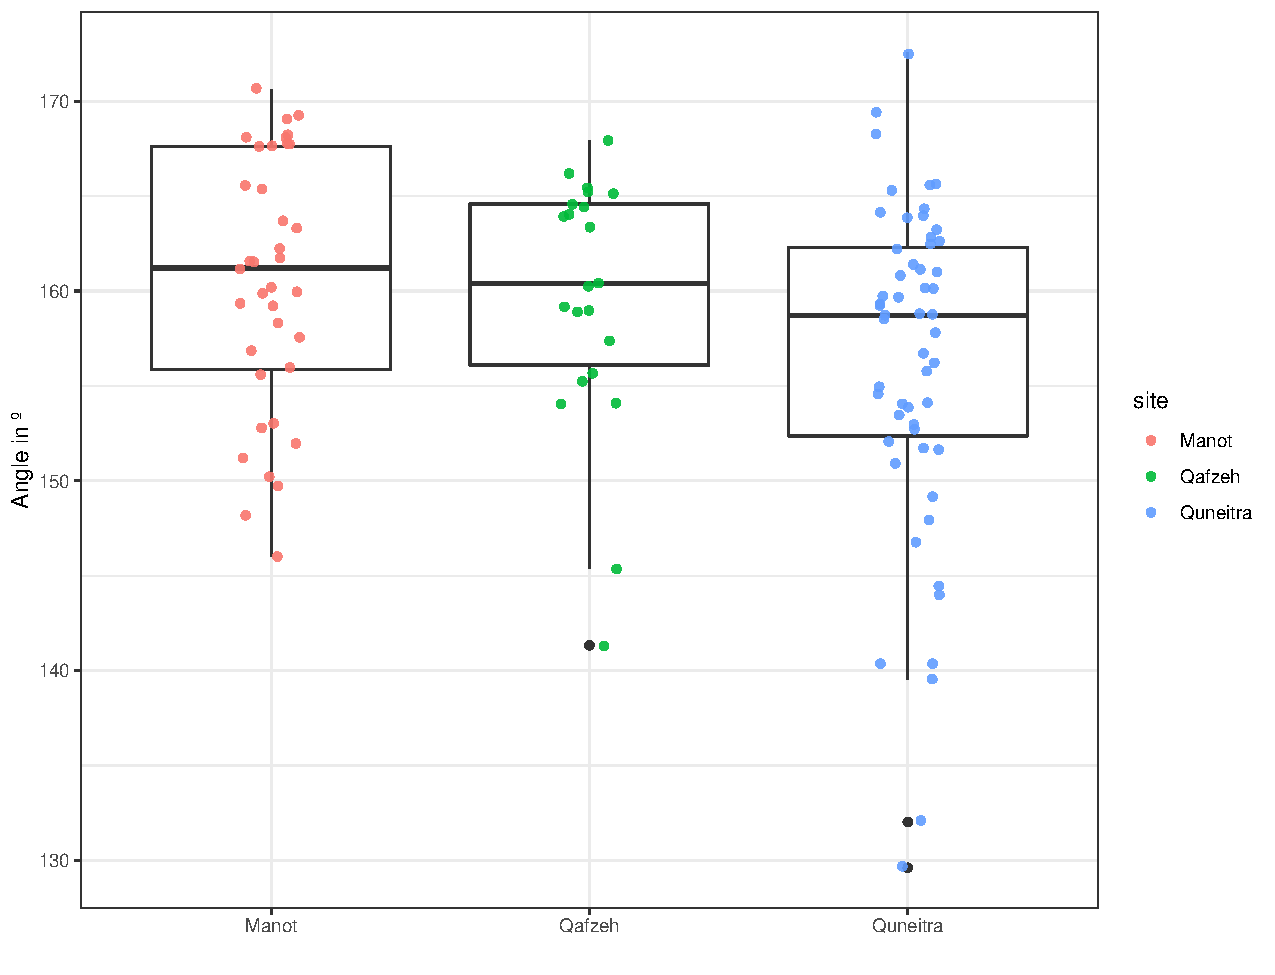
\includegraphics{incisionangles_files/figure-latex/unnamed-chunk-5-1.pdf}

\begin{Shaded}
\begin{Highlighting}[]
\FunctionTok{hist}\NormalTok{(onewaymodeldepth}\SpecialCharTok{$}\NormalTok{residuals)}
\end{Highlighting}
\end{Shaded}

\includegraphics{incisionangles_files/figure-latex/unnamed-chunk-5-2.pdf}

\begin{Shaded}
\begin{Highlighting}[]
\FunctionTok{hist}\NormalTok{(onewaymodelarea}\SpecialCharTok{$}\NormalTok{residuals)}
\end{Highlighting}
\end{Shaded}

\includegraphics{incisionangles_files/figure-latex/unnamed-chunk-5-3.pdf}

\begin{Shaded}
\begin{Highlighting}[]
\FunctionTok{hist}\NormalTok{(onewaymodelangle}\SpecialCharTok{$}\NormalTok{residuals)}
\end{Highlighting}
\end{Shaded}

\includegraphics{incisionangles_files/figure-latex/unnamed-chunk-5-4.pdf}

\begin{Shaded}
\begin{Highlighting}[]
\CommentTok{\# library(car)}
\FunctionTok{qqPlot}\NormalTok{(onewaymodelwidth}\SpecialCharTok{$}\NormalTok{residuals)}
\end{Highlighting}
\end{Shaded}

\includegraphics{incisionangles_files/figure-latex/unnamed-chunk-5-5.pdf}

\begin{verbatim}
## [1] 224 215
\end{verbatim}

\begin{Shaded}
\begin{Highlighting}[]
\FunctionTok{qqPlot}\NormalTok{(onewaymodeldepth}\SpecialCharTok{$}\NormalTok{residuals)}
\end{Highlighting}
\end{Shaded}

\includegraphics{incisionangles_files/figure-latex/unnamed-chunk-5-6.pdf}

\begin{verbatim}
## [1] 225  59
\end{verbatim}

\begin{Shaded}
\begin{Highlighting}[]
\FunctionTok{qqPlot}\NormalTok{(onewaymodelarea}\SpecialCharTok{$}\NormalTok{residuals)}
\end{Highlighting}
\end{Shaded}

\includegraphics{incisionangles_files/figure-latex/unnamed-chunk-5-7.pdf}

\begin{verbatim}
## [1] 225 224
\end{verbatim}

\begin{Shaded}
\begin{Highlighting}[]
\FunctionTok{qqPlot}\NormalTok{(onewaymodelangle}\SpecialCharTok{$}\NormalTok{residuals)}
\end{Highlighting}
\end{Shaded}

\includegraphics{incisionangles_files/figure-latex/unnamed-chunk-5-8.pdf}

\begin{verbatim}
## [1] 167 225
\end{verbatim}

\begin{Shaded}
\begin{Highlighting}[]
\CommentTok{\# check if model fits the assumption, the homogeneity of variances}
\FunctionTok{par}\NormalTok{(}\AttributeTok{mfrow=}\FunctionTok{c}\NormalTok{(}\DecValTok{2}\NormalTok{,}\DecValTok{2}\NormalTok{))}
\FunctionTok{plot}\NormalTok{(onewaymodelwidth)}
\end{Highlighting}
\end{Shaded}

\includegraphics{incisionangles_files/figure-latex/unnamed-chunk-5-9.pdf}

\begin{Shaded}
\begin{Highlighting}[]
\FunctionTok{par}\NormalTok{(}\AttributeTok{mfrow=}\FunctionTok{c}\NormalTok{(}\DecValTok{1}\NormalTok{,}\DecValTok{1}\NormalTok{))}

\FunctionTok{par}\NormalTok{(}\AttributeTok{mfrow=}\FunctionTok{c}\NormalTok{(}\DecValTok{2}\NormalTok{,}\DecValTok{2}\NormalTok{))}
\FunctionTok{plot}\NormalTok{(onewaymodeldepth)}
\end{Highlighting}
\end{Shaded}

\includegraphics{incisionangles_files/figure-latex/unnamed-chunk-5-10.pdf}

\begin{Shaded}
\begin{Highlighting}[]
\FunctionTok{par}\NormalTok{(}\AttributeTok{mfrow=}\FunctionTok{c}\NormalTok{(}\DecValTok{1}\NormalTok{,}\DecValTok{1}\NormalTok{))}

\FunctionTok{par}\NormalTok{(}\AttributeTok{mfrow=}\FunctionTok{c}\NormalTok{(}\DecValTok{2}\NormalTok{,}\DecValTok{2}\NormalTok{))}
\FunctionTok{plot}\NormalTok{(onewaymodelarea)}
\end{Highlighting}
\end{Shaded}

\includegraphics{incisionangles_files/figure-latex/unnamed-chunk-5-11.pdf}

\begin{Shaded}
\begin{Highlighting}[]
\FunctionTok{par}\NormalTok{(}\AttributeTok{mfrow=}\FunctionTok{c}\NormalTok{(}\DecValTok{1}\NormalTok{,}\DecValTok{1}\NormalTok{))}

\FunctionTok{par}\NormalTok{(}\AttributeTok{mfrow=}\FunctionTok{c}\NormalTok{(}\DecValTok{2}\NormalTok{,}\DecValTok{2}\NormalTok{))}
\FunctionTok{plot}\NormalTok{(onewaymodelangle)}
\end{Highlighting}
\end{Shaded}

\includegraphics{incisionangles_files/figure-latex/unnamed-chunk-5-12.pdf}

\begin{Shaded}
\begin{Highlighting}[]
\FunctionTok{par}\NormalTok{(}\AttributeTok{mfrow=}\FunctionTok{c}\NormalTok{(}\DecValTok{1}\NormalTok{,}\DecValTok{1}\NormalTok{))}

\CommentTok{\# The model fits the assumption of homoscedasticity}

\CommentTok{\# ANOVA tells us if there are differences among group means (sites and features), but not where those differences are. To find out which groups are statistically different from one another, you perform a Tukey’s Honestly Significant Difference Tukey’s HSD post{-}hoc test for pairwise comparisons.}

\CommentTok{\# check which groups are statistically different from one another}
\FunctionTok{TukeyHSD}\NormalTok{(onewaymodelwidth, }\AttributeTok{conf.level=}\NormalTok{.}\DecValTok{95}\NormalTok{) }
\end{Highlighting}
\end{Shaded}

\begin{verbatim}
##   Tukey multiple comparisons of means
##     95% family-wise confidence level
## 
## Fit: aov(formula = horizontaldistance ~ site, data = db)
## 
## $site
##                      diff       lwr       upr     p adj
## Amud2-Amud1     -31.13481 -93.73121  31.46158 0.6508190
## Manot-Amud1     435.00665 368.94828 501.06502 0.0000000
## Qafzeh-Amud1    607.55586 517.69281 697.41890 0.0000000
## Quneitra-Amud1  631.97252 559.62870 704.31634 0.0000000
## Manot-Amud2     466.14146 394.57268 537.71024 0.0000000
## Qafzeh-Amud2    638.69067 544.70264 732.67870 0.0000000
## Quneitra-Amud2  663.10733 585.69926 740.51541 0.0000000
## Qafzeh-Manot    172.54921  76.22087 268.87755 0.0000141
## Quneitra-Manot  196.96587 116.73240 277.19934 0.0000000
## Quneitra-Qafzeh  24.41667 -76.32592 125.15926 0.9637087
\end{verbatim}

\begin{Shaded}
\begin{Highlighting}[]
\FunctionTok{plot}\NormalTok{(}\FunctionTok{TukeyHSD}\NormalTok{(onewaymodelwidth, }\AttributeTok{conf.level=}\NormalTok{.}\DecValTok{95}\NormalTok{), }\AttributeTok{las =} \DecValTok{1}\NormalTok{, }\AttributeTok{cex.axis=}\FloatTok{0.5}\NormalTok{)}
\end{Highlighting}
\end{Shaded}

\includegraphics{incisionangles_files/figure-latex/unnamed-chunk-5-13.pdf}

\begin{Shaded}
\begin{Highlighting}[]
\FunctionTok{TukeyHSD}\NormalTok{(onewaymodeldepth, }\AttributeTok{conf.level=}\NormalTok{.}\DecValTok{95}\NormalTok{) }
\end{Highlighting}
\end{Shaded}

\begin{verbatim}
##   Tukey multiple comparisons of means
##     95% family-wise confidence level
## 
## Fit: aov(formula = maximumdepth ~ site, data = db)
## 
## $site
##                      diff        lwr       upr     p adj
## Amud2-Amud1     -4.119425 -18.028363  9.789513 0.9266782
## Manot-Amud1     24.027616   9.349427 38.705805 0.0000966
## Qafzeh-Amud1    30.536664  10.569067 50.504260 0.0003391
## Quneitra-Amud1  70.100691  54.025873 86.175510 0.0000000
## Manot-Amud2     28.147041  12.244437 44.049646 0.0000185
## Qafzeh-Amud2    34.656089  13.771920 55.540257 0.0000736
## Quneitra-Amud2  74.220117  57.020019 91.420215 0.0000000
## Qafzeh-Manot     6.509048 -14.895138 27.913233 0.9198008
## Quneitra-Manot  46.073075  28.245175 63.900976 0.0000000
## Quneitra-Qafzeh 39.564028  17.178994 61.949061 0.0000191
\end{verbatim}

\begin{Shaded}
\begin{Highlighting}[]
\FunctionTok{plot}\NormalTok{(}\FunctionTok{TukeyHSD}\NormalTok{(onewaymodeldepth, }\AttributeTok{conf.level=}\NormalTok{.}\DecValTok{95}\NormalTok{), }\AttributeTok{las =} \DecValTok{1}\NormalTok{, }\AttributeTok{cex.axis=}\FloatTok{0.5}\NormalTok{)}
\end{Highlighting}
\end{Shaded}

\includegraphics{incisionangles_files/figure-latex/unnamed-chunk-5-14.pdf}

\begin{Shaded}
\begin{Highlighting}[]
\FunctionTok{TukeyHSD}\NormalTok{(onewaymodelarea, }\AttributeTok{conf.level=}\NormalTok{.}\DecValTok{95}\NormalTok{) }
\end{Highlighting}
\end{Shaded}

\begin{verbatim}
##   Tukey multiple comparisons of means
##     95% family-wise confidence level
## 
## Fit: aov(formula = holearea ~ site, data = db)
## 
## $site
##                      diff        lwr      upr     p adj
## Amud2-Amud1     -1790.275 -13697.294 10116.74 0.9939065
## Manot-Amud1     18903.955   6338.403 31469.51 0.0004484
## Qafzeh-Amud1    29737.055  12643.403 46830.71 0.0000272
## Quneitra-Amud1  64322.435  50561.272 78083.60 0.0000000
## Manot-Amud2     20694.230   7080.494 34307.97 0.0003762
## Qafzeh-Amud2    31527.330  13649.029 49405.63 0.0000201
## Quneitra-Amud2  66112.710  51388.229 80837.19 0.0000000
## Qafzeh-Manot    10833.101  -7490.372 29156.57 0.4844187
## Quneitra-Manot  45418.480  30156.556 60680.40 0.0000000
## Quneitra-Qafzeh 34585.380  15422.233 53748.53 0.0000118
\end{verbatim}

\begin{Shaded}
\begin{Highlighting}[]
\FunctionTok{plot}\NormalTok{(}\FunctionTok{TukeyHSD}\NormalTok{(onewaymodelarea, }\AttributeTok{conf.level=}\NormalTok{.}\DecValTok{95}\NormalTok{), }\AttributeTok{las =} \DecValTok{1}\NormalTok{, }\AttributeTok{cex.axis=}\FloatTok{0.5}\NormalTok{)}
\end{Highlighting}
\end{Shaded}

\includegraphics{incisionangles_files/figure-latex/unnamed-chunk-5-15.pdf}

\begin{Shaded}
\begin{Highlighting}[]
\FunctionTok{TukeyHSD}\NormalTok{(onewaymodelangle, }\AttributeTok{conf.level=}\NormalTok{.}\DecValTok{95}\NormalTok{) }
\end{Highlighting}
\end{Shaded}

\begin{verbatim}
##   Tukey multiple comparisons of means
##     95% family-wise confidence level
## 
## Fit: aov(formula = angle ~ site, data = db)
## 
## $site
##                       diff        lwr        upr     p adj
## Amud2-Amud1      3.9949550   1.039992  6.9499179 0.0022690
## Manot-Amud1     -4.4926641  -7.611055 -1.3742732 0.0009003
## Qafzeh-Amud1    -4.7894895  -9.031618 -0.5473606 0.0179890
## Quneitra-Amud1  -5.3304617  -8.745567 -1.9153561 0.0002366
## Manot-Amud2     -8.4876190 -11.866138 -5.1091004 0.0000000
## Qafzeh-Amud2    -8.7844444 -13.221300 -4.3475892 0.0000011
## Quneitra-Amud2  -9.3254167 -12.979589 -5.6712446 0.0000000
## Qafzeh-Manot    -0.2968254  -4.844159  4.2505079 0.9997691
## Quneitra-Manot  -0.8377976  -4.625347  2.9497516 0.9739556
## Quneitra-Qafzeh -0.5409722  -5.296687  4.2147428 0.9979346
\end{verbatim}

\begin{Shaded}
\begin{Highlighting}[]
\FunctionTok{plot}\NormalTok{(}\FunctionTok{TukeyHSD}\NormalTok{(onewaymodelangle, }\AttributeTok{conf.level=}\NormalTok{.}\DecValTok{95}\NormalTok{), }\AttributeTok{las =} \DecValTok{1}\NormalTok{, }\AttributeTok{cex.axis=}\FloatTok{0.5}\NormalTok{)}
\end{Highlighting}
\end{Shaded}

\includegraphics{incisionangles_files/figure-latex/unnamed-chunk-5-16.pdf}

\begin{Shaded}
\begin{Highlighting}[]
\CommentTok{\# Some observations from the post{-}hoc test results:}
\CommentTok{\# All raw materials are significantly different from each other. All p{-}value (here represented as p adj) are smaller than 0.05.}
\end{Highlighting}
\end{Shaded}

\begin{center}\rule{0.5\linewidth}{0.5pt}\end{center}

End of Script

\end{document}
